\chapter{Additional Fake Rate Material}\label{ch:appendix_fake_rate}


\section{The MC Fake Rate Fits}\label{sec:mc_fake_rate_fits}

The \sieie template fits used in the MC based closure test to the photon fake rate method are shown in Fig.~\ref{fig:all_mc_sieie_fits} for the EB and EE regions. The fits are performed in photon \pt bins of 50-70, 70-90, 90-130, 130-200, and 200-600\GeV. The nominal sideband definition of $5 < \chiso < 10\GeV$ is used for both categories. These same plots were produced after inverting the template and sideband variables. The \chiso template fits are shown in Fig.~\ref{fig:all_mc_chiso_fits} for the EB and EE regions. The fits are performed in the same photon \pt bins, using the nominal sideband of $0.0105 < \sieie < 0.0150$ in the EB and $0.0280 < \sieie < 0.0400$ in the EE category.

\begin{figure}[!htbp]
	\noindent
	\centering
	\begin{multicols}{2}
		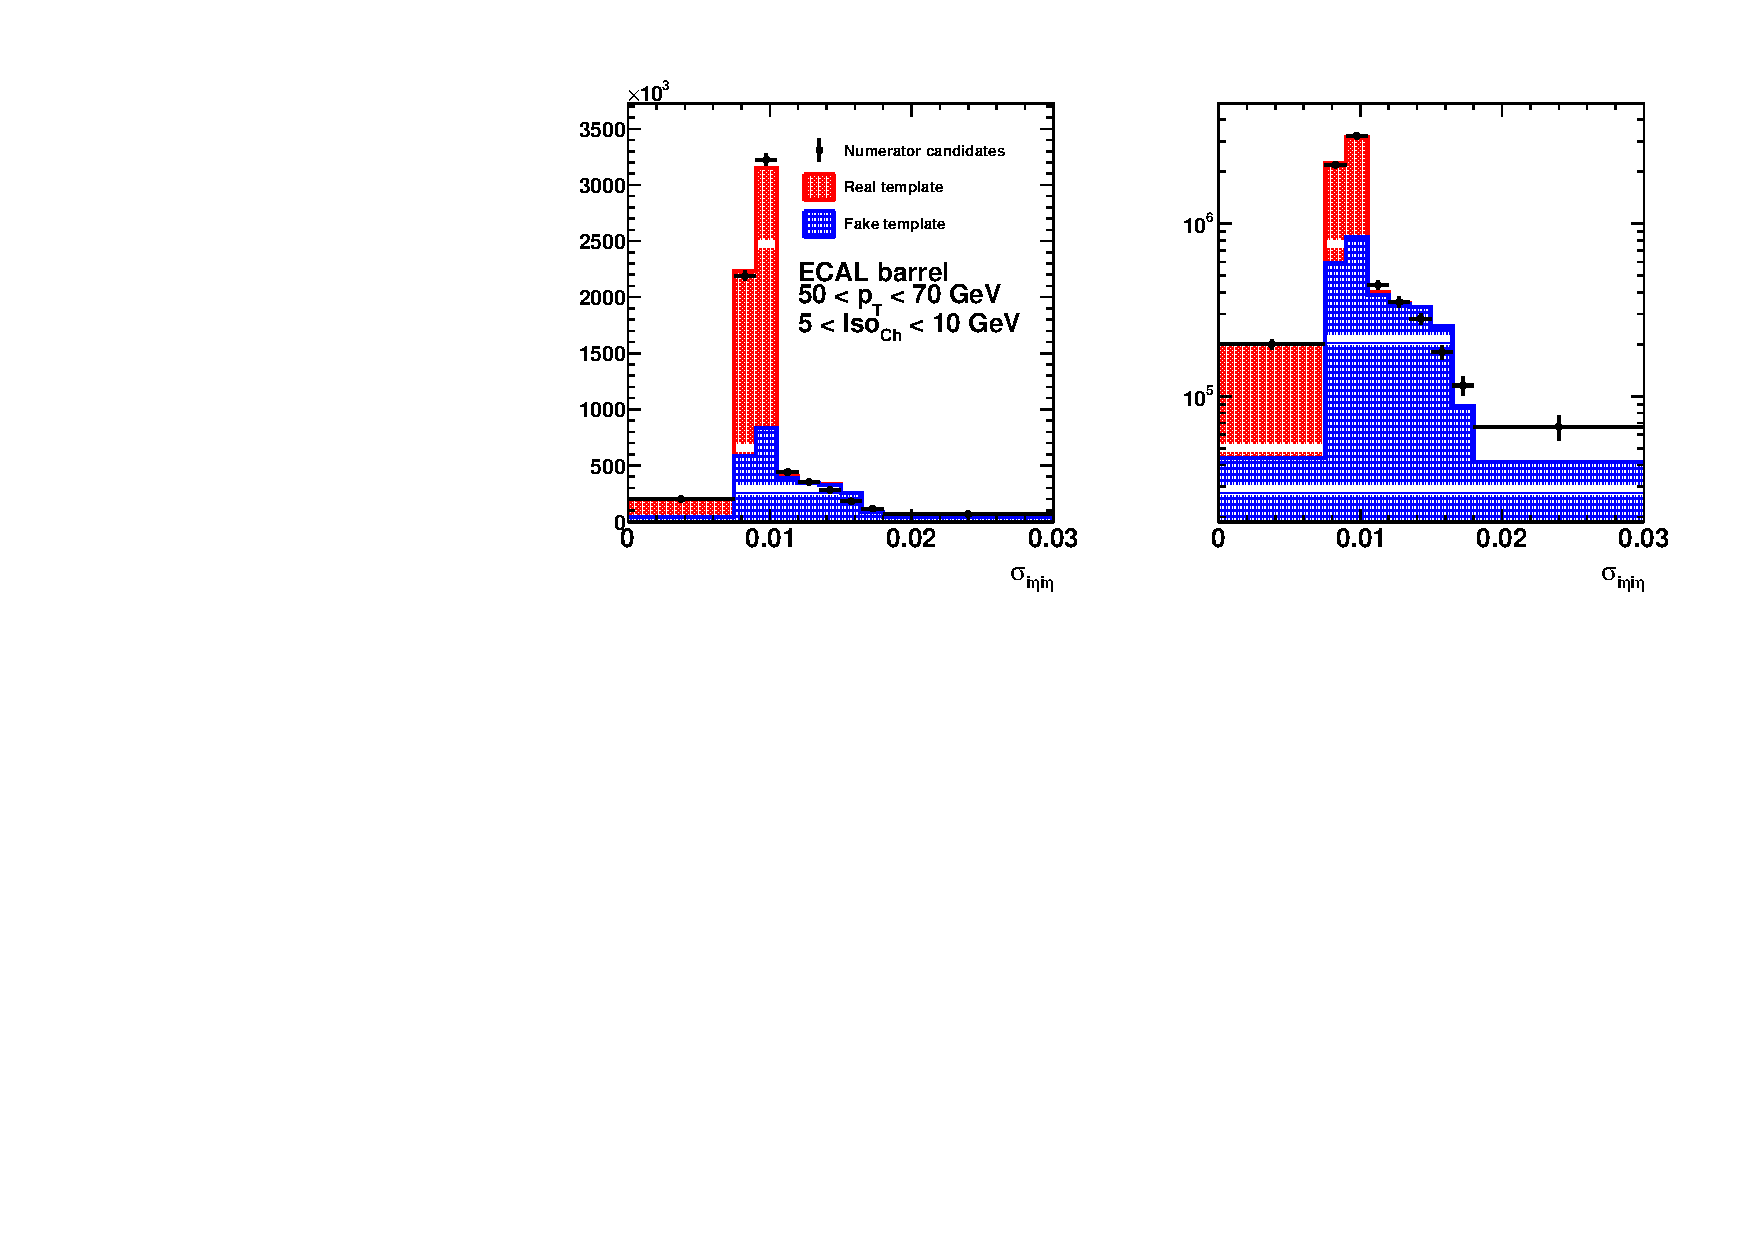
\includegraphics[scale=0.41]{figures/closure_test_h_pt50To70_chIso5To10_EB_Fake_sieie.pdf} \\
		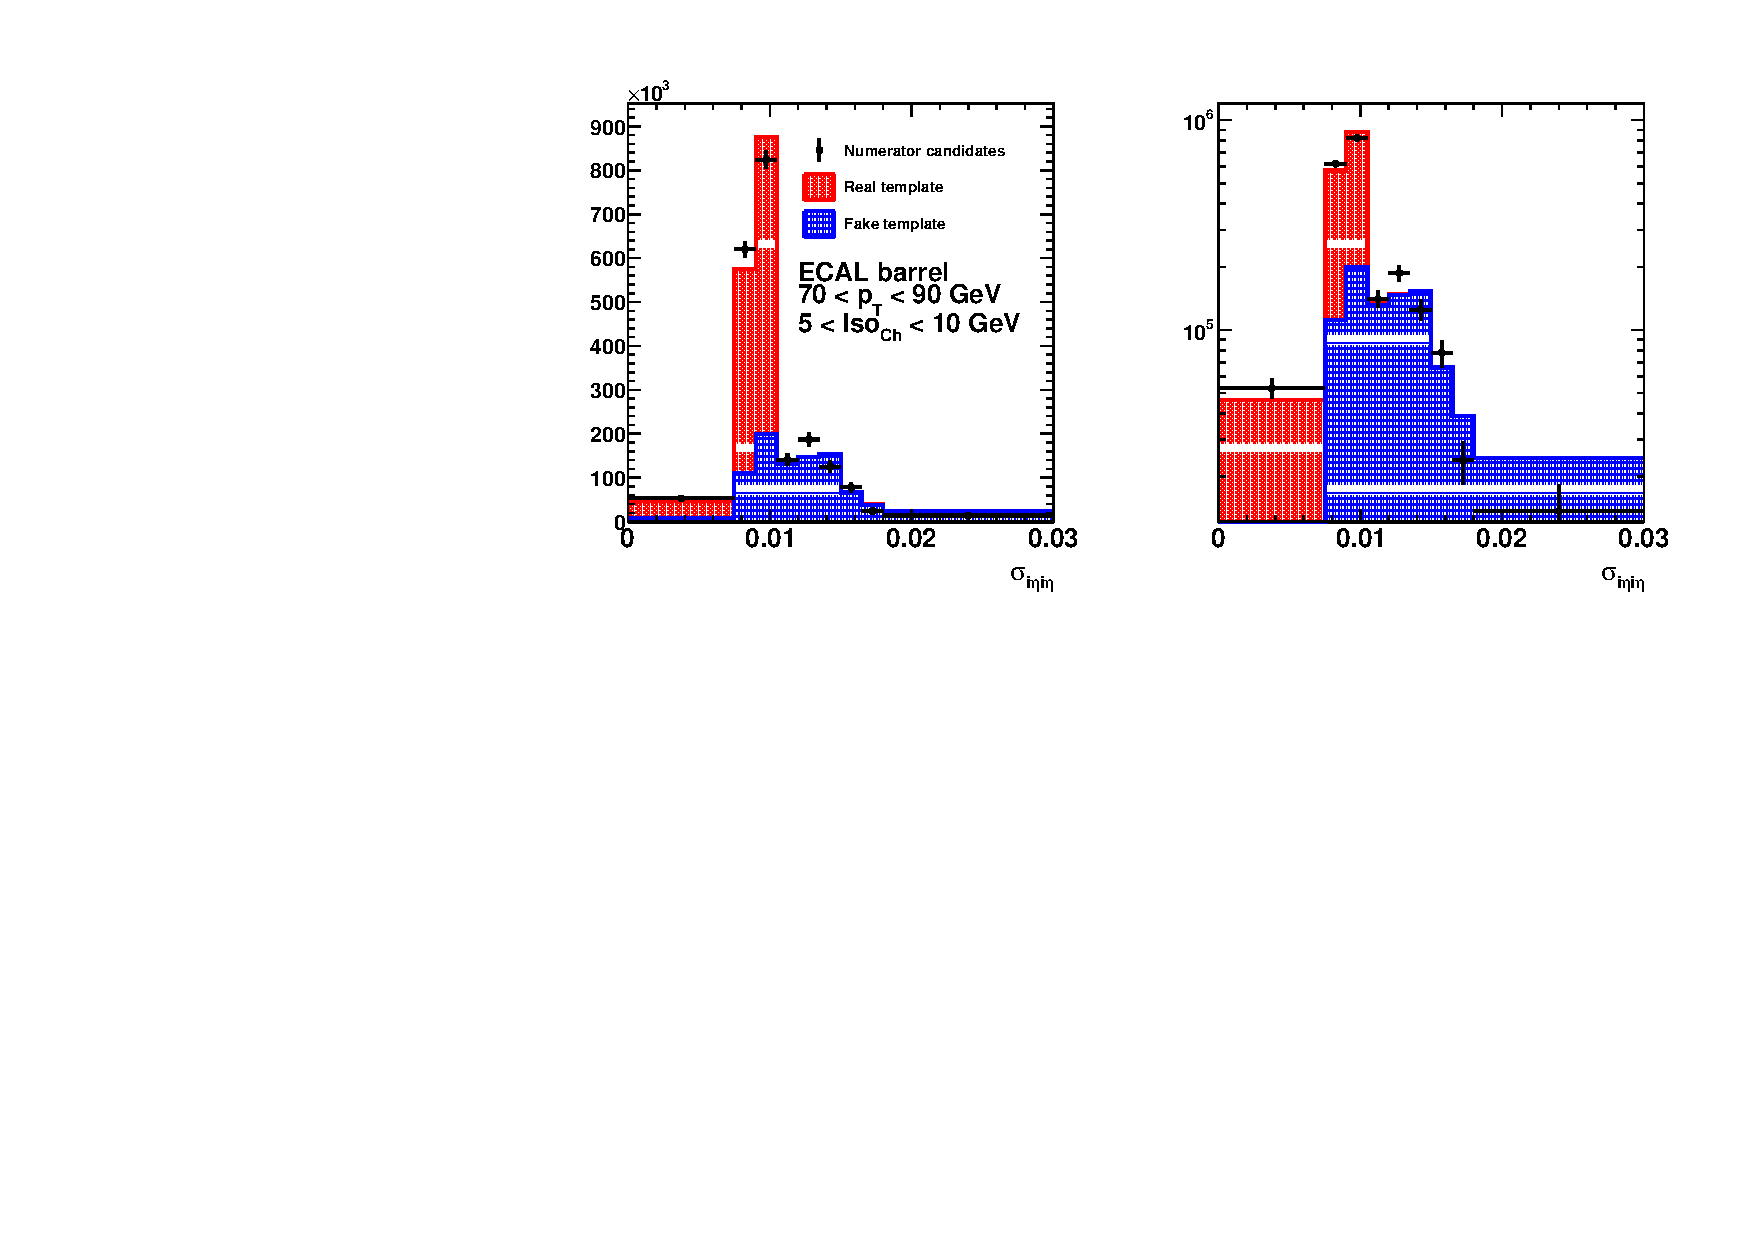
\includegraphics[scale=0.41]{figures/closure_test_h_pt70To90_chIso5To10_EB_Fake_sieie.pdf} \\
		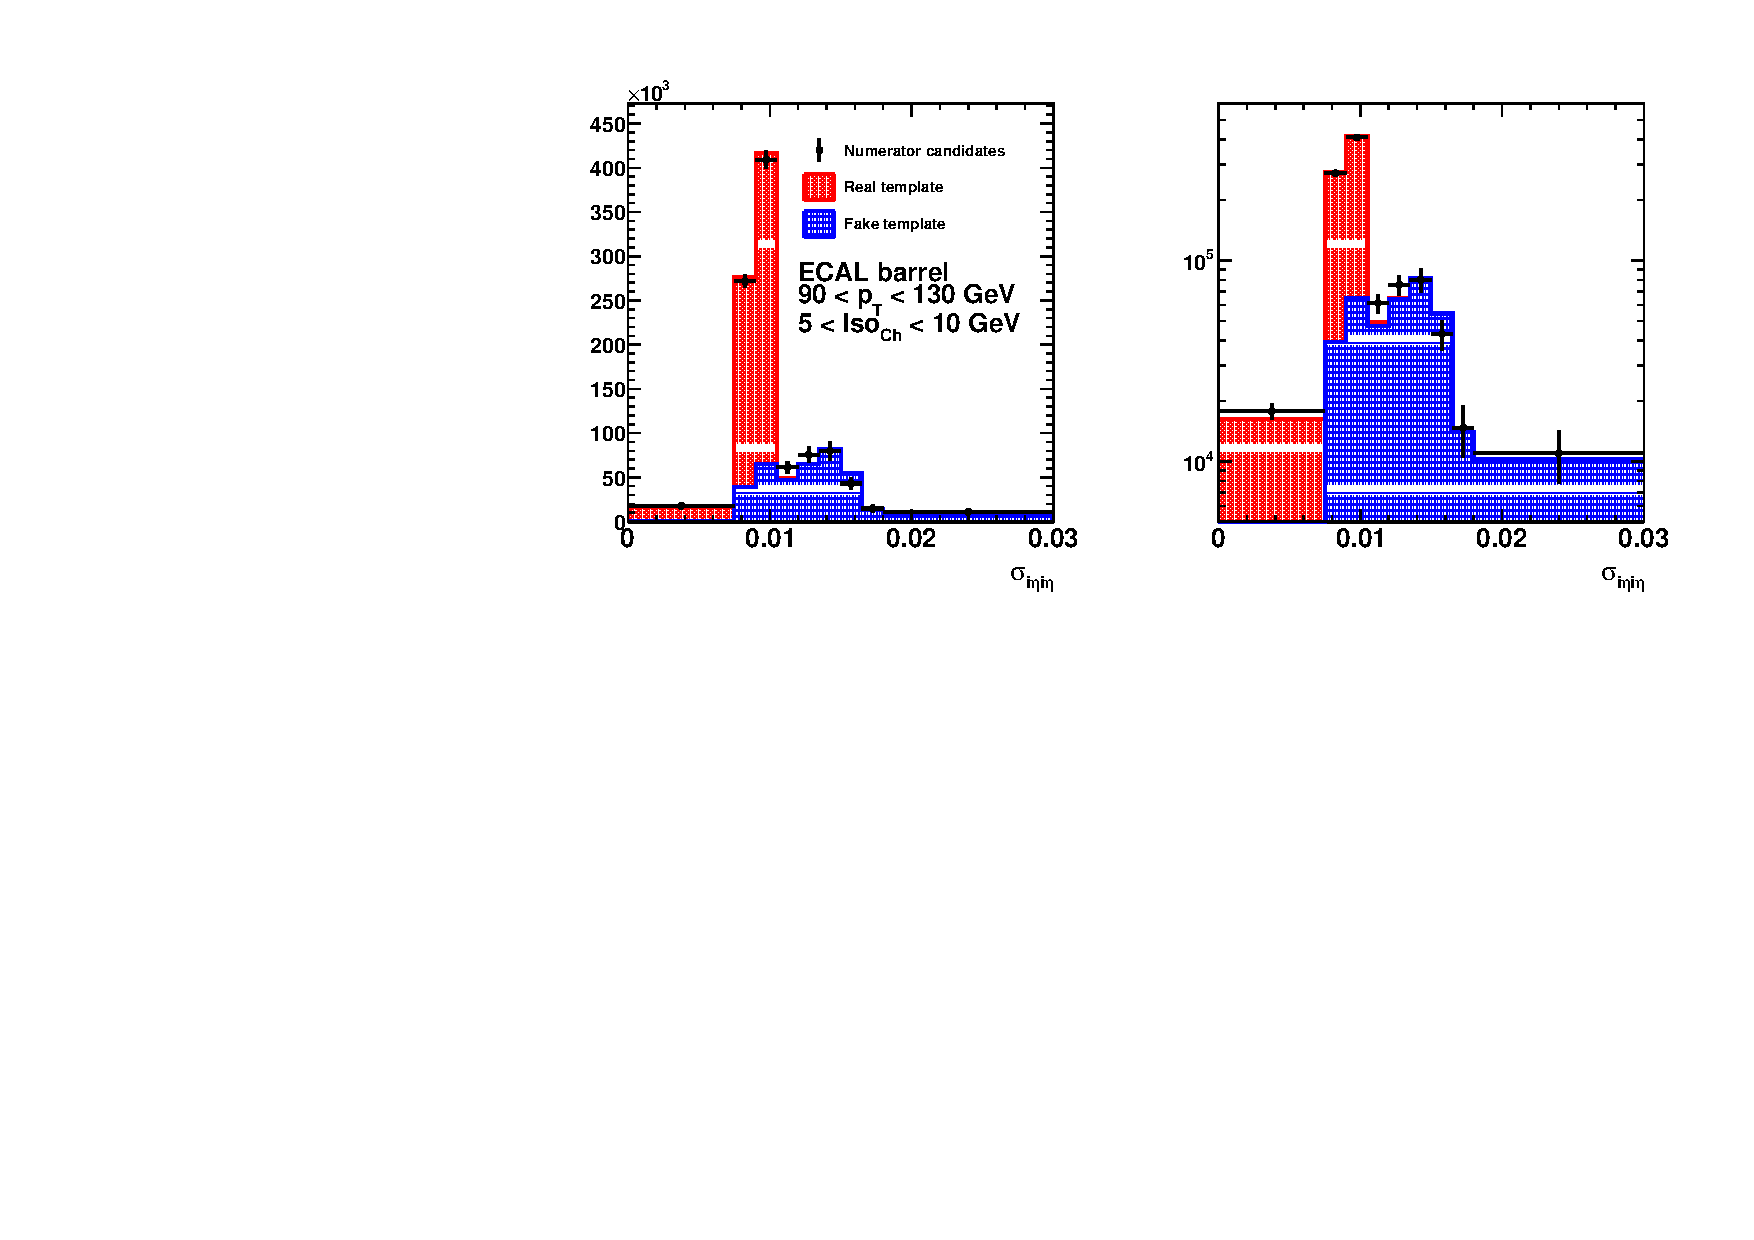
\includegraphics[scale=0.41]{figures/closure_test_h_pt90To130_chIso5To10_EB_Fake_sieie.pdf} \\
		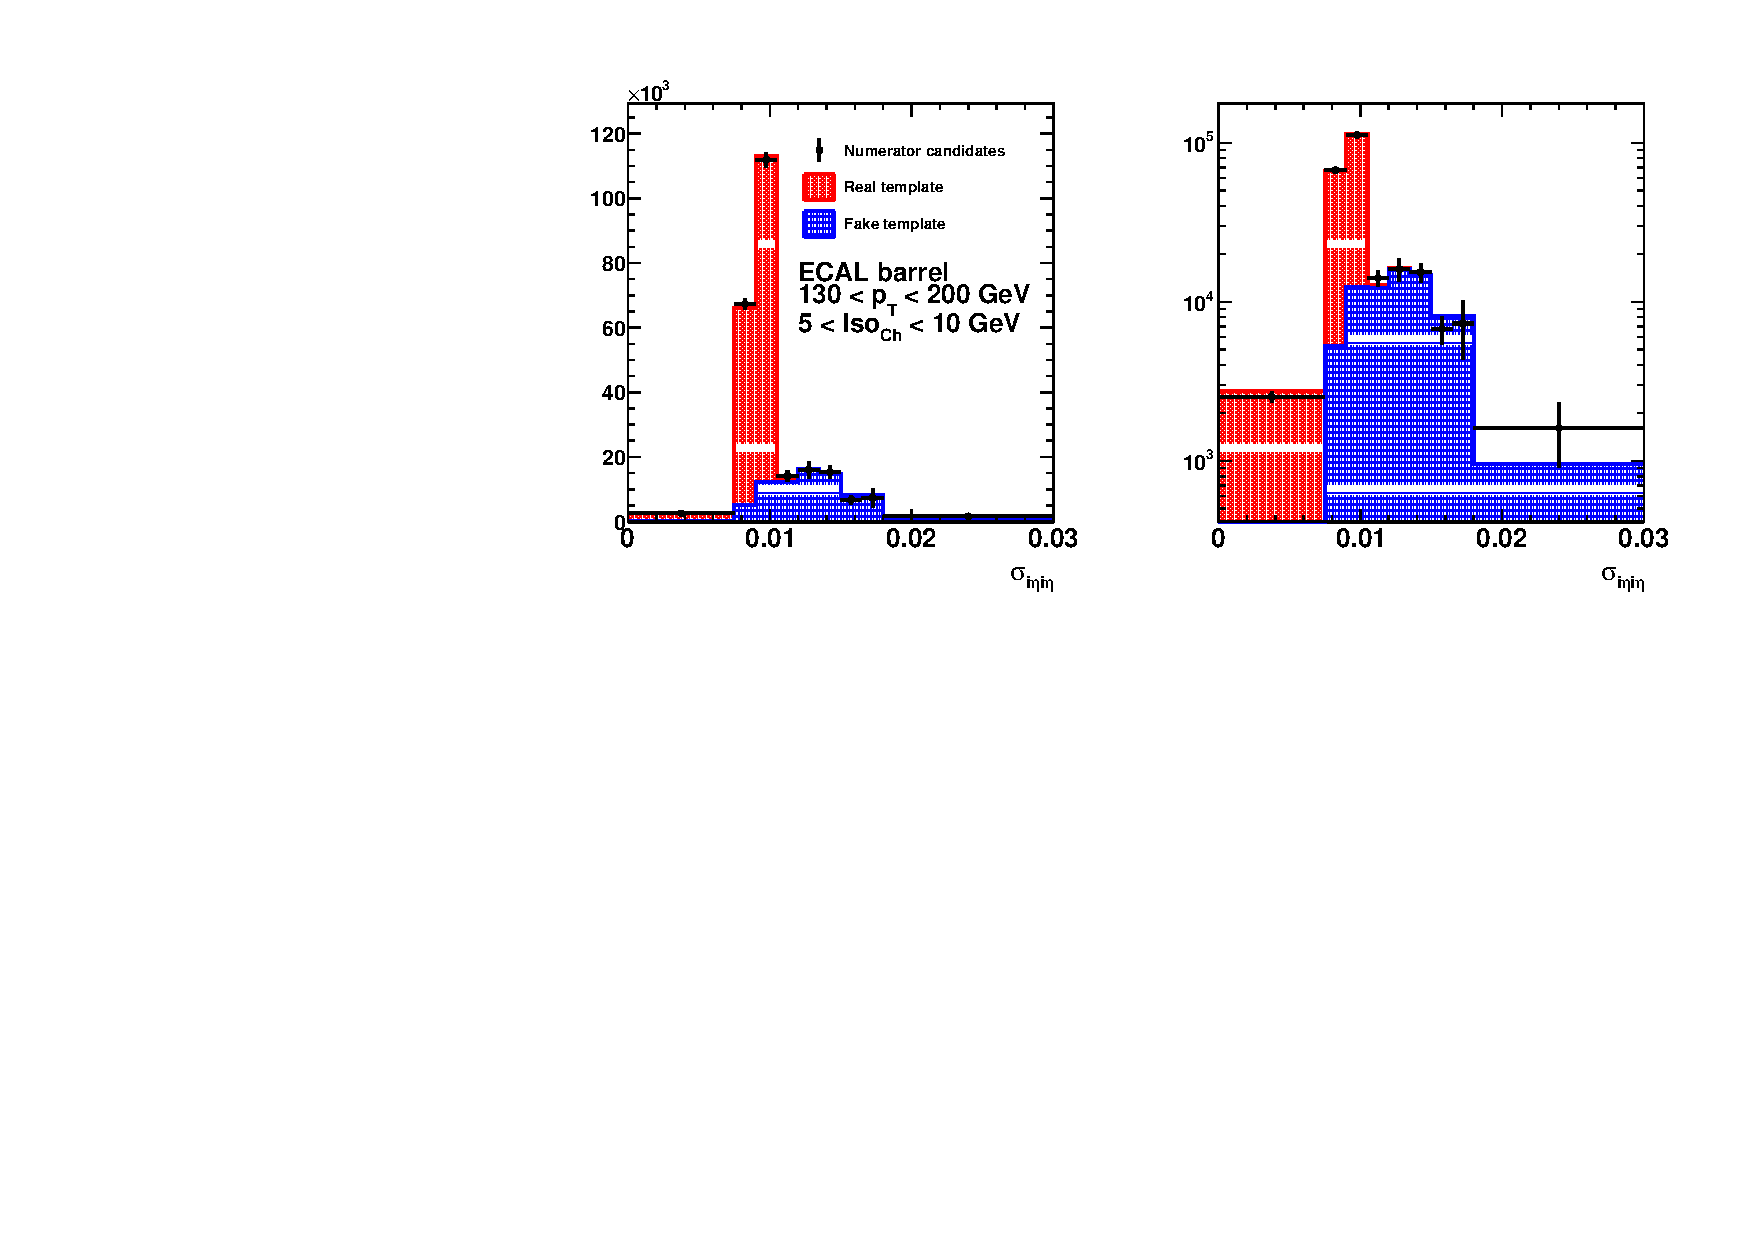
\includegraphics[scale=0.41]{figures/closure_test_h_pt130To200_chIso5To10_EB_Fake_sieie.pdf} \\
		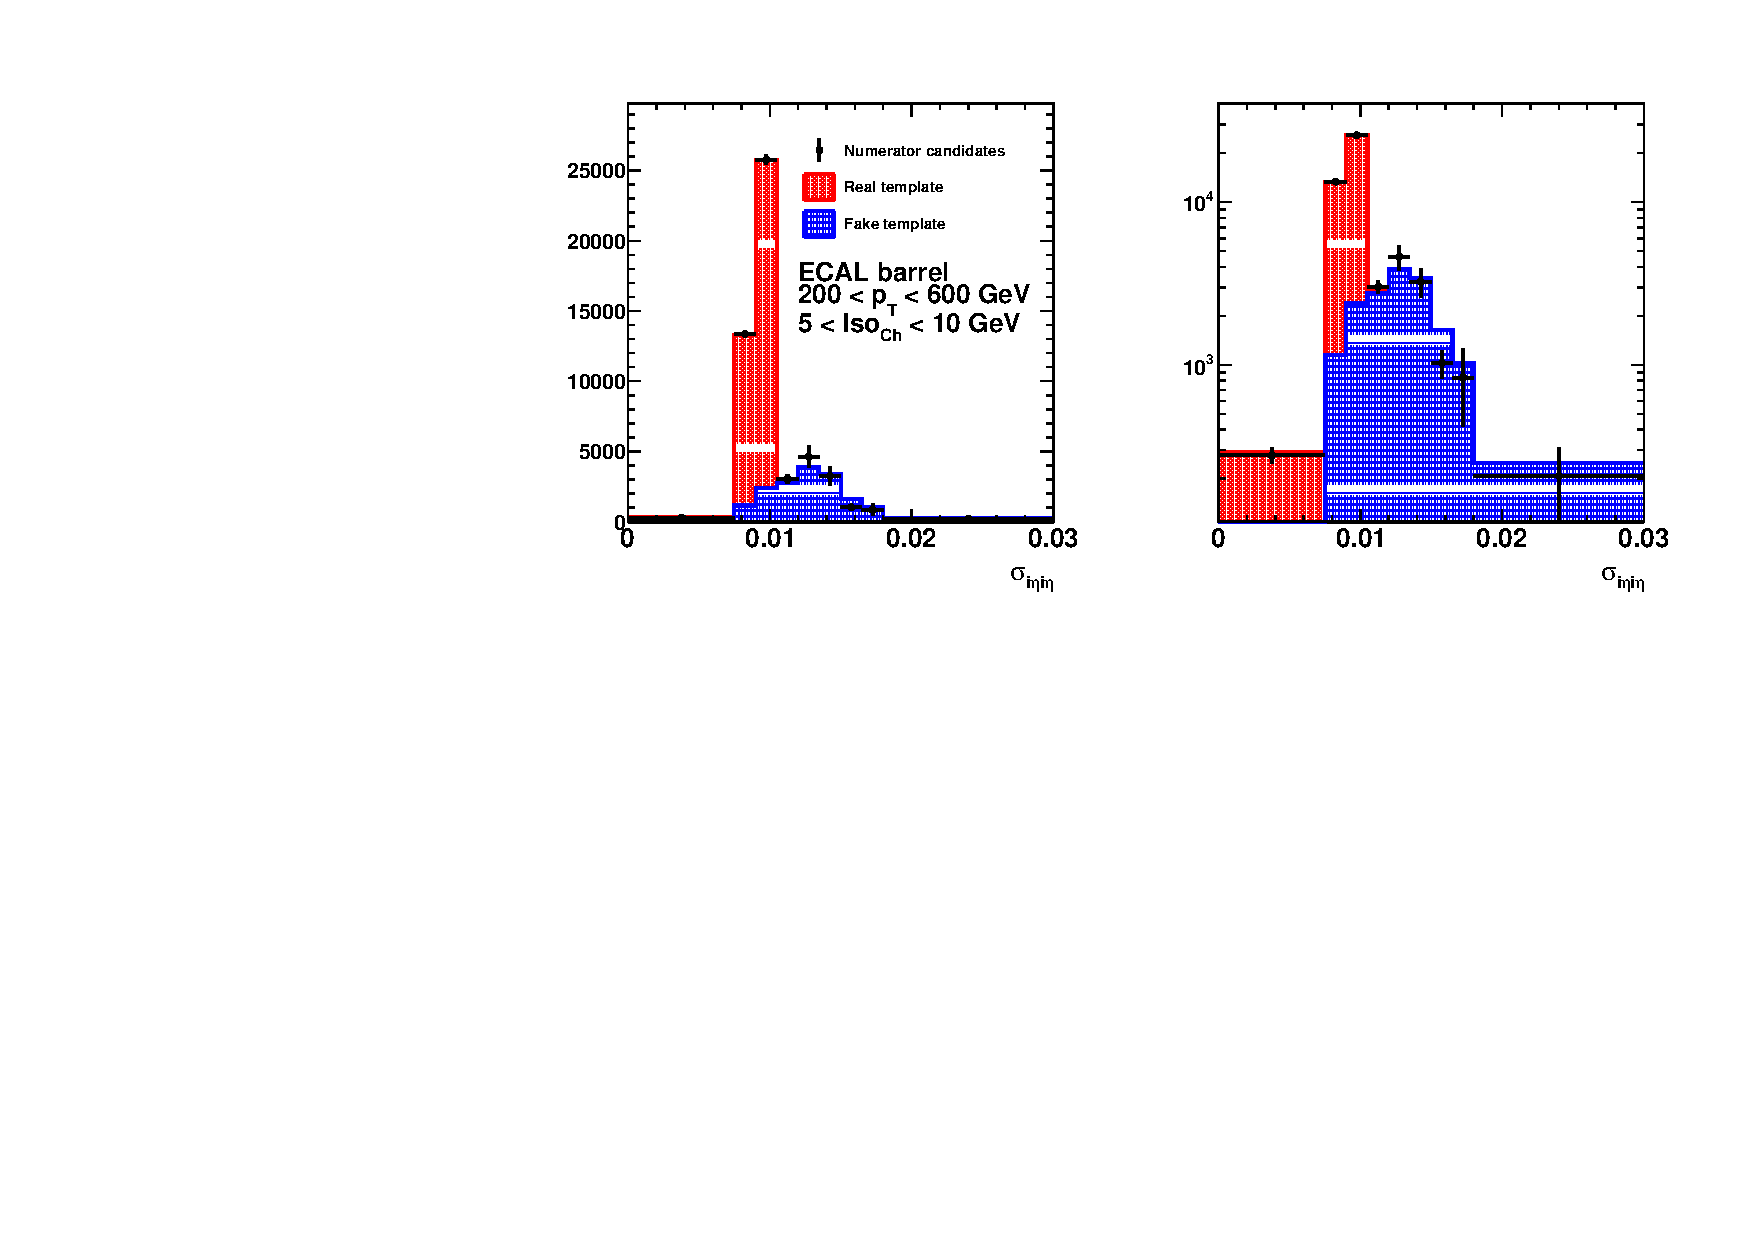
\includegraphics[scale=0.41]{figures/closure_test_h_pt200To600_chIso5To10_EB_Fake_sieie.pdf} \\
		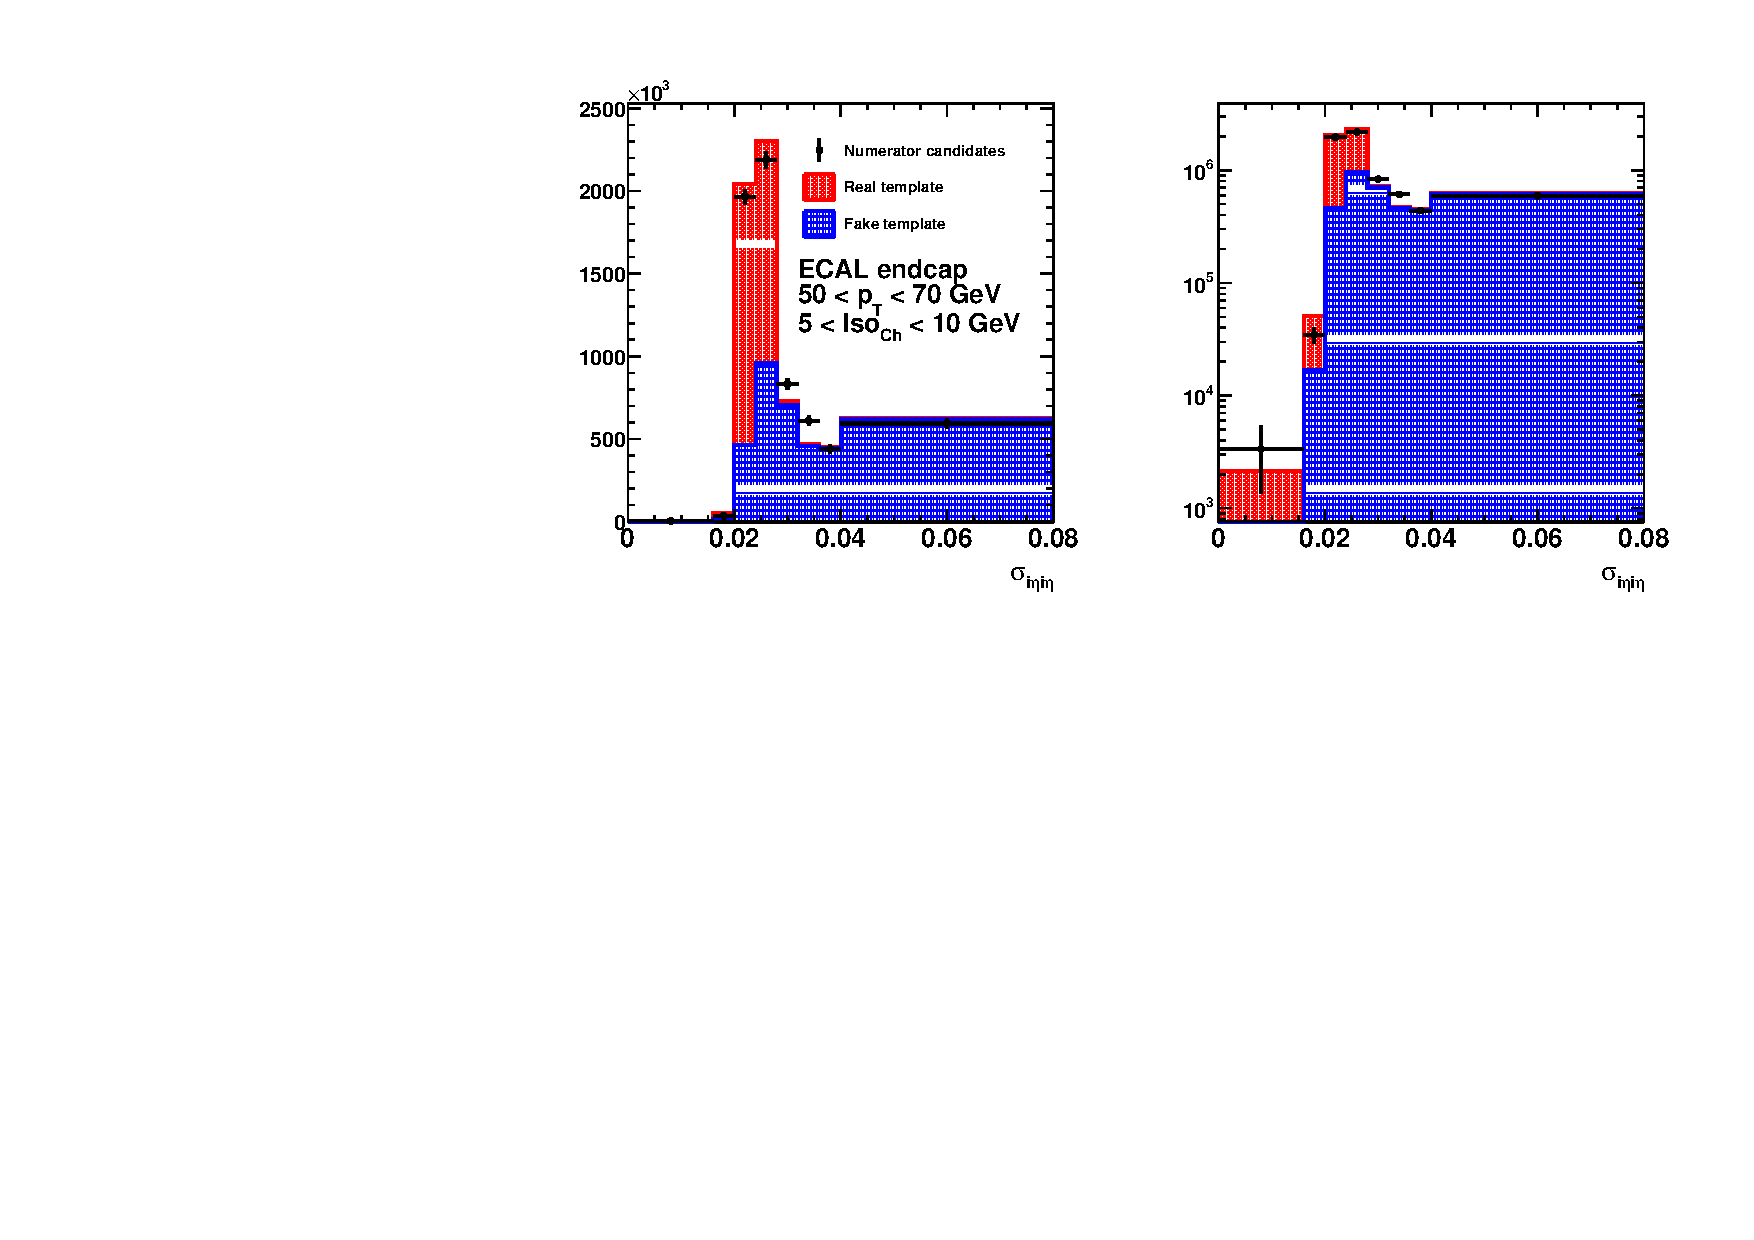
\includegraphics[scale=0.41]{figures/closure_test_h_pt50To70_chIso5To10_EE_Fake_sieie.pdf} \\
		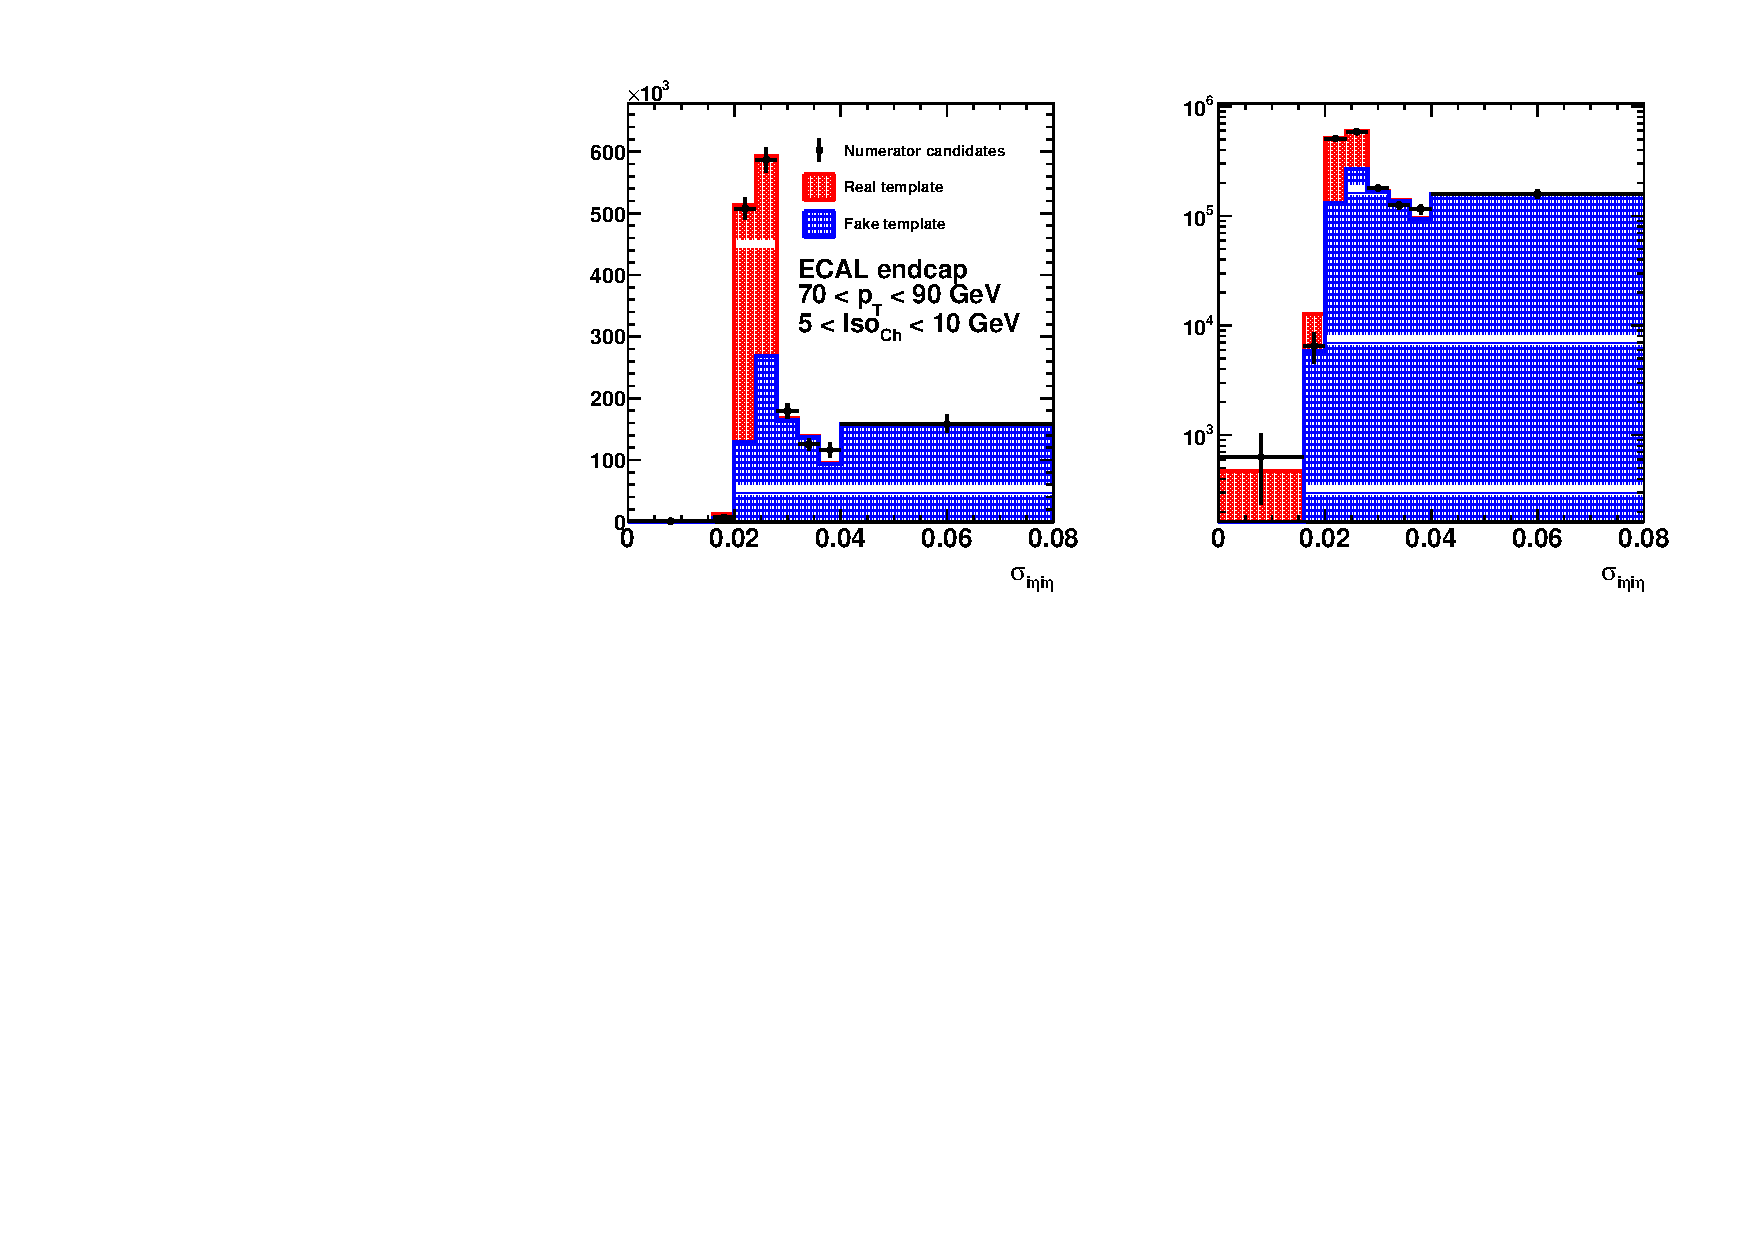
\includegraphics[scale=0.41]{figures/closure_test_h_pt70To90_chIso5To10_EE_Fake_sieie.pdf} \\
		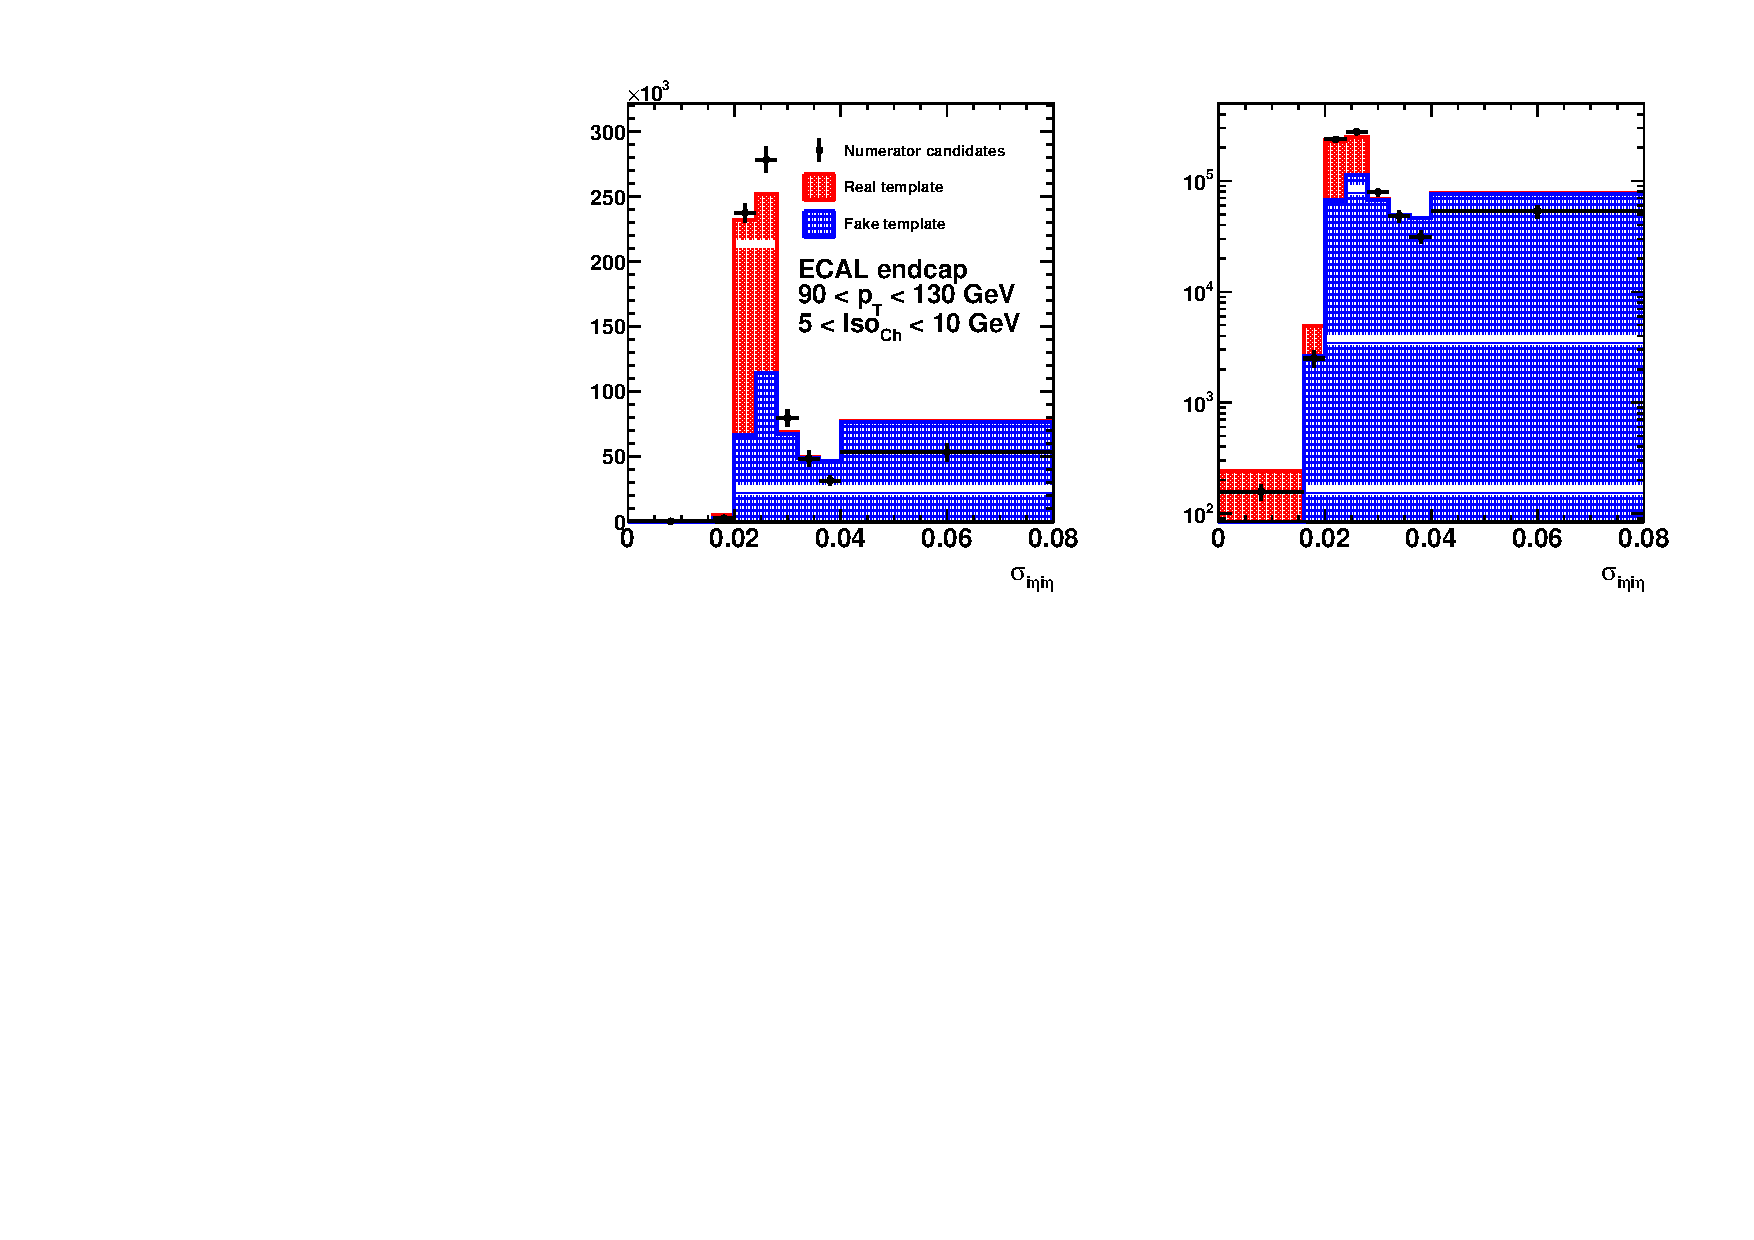
\includegraphics[scale=0.41]{figures/closure_test_h_pt90To130_chIso5To10_EE_Fake_sieie.pdf} \\
		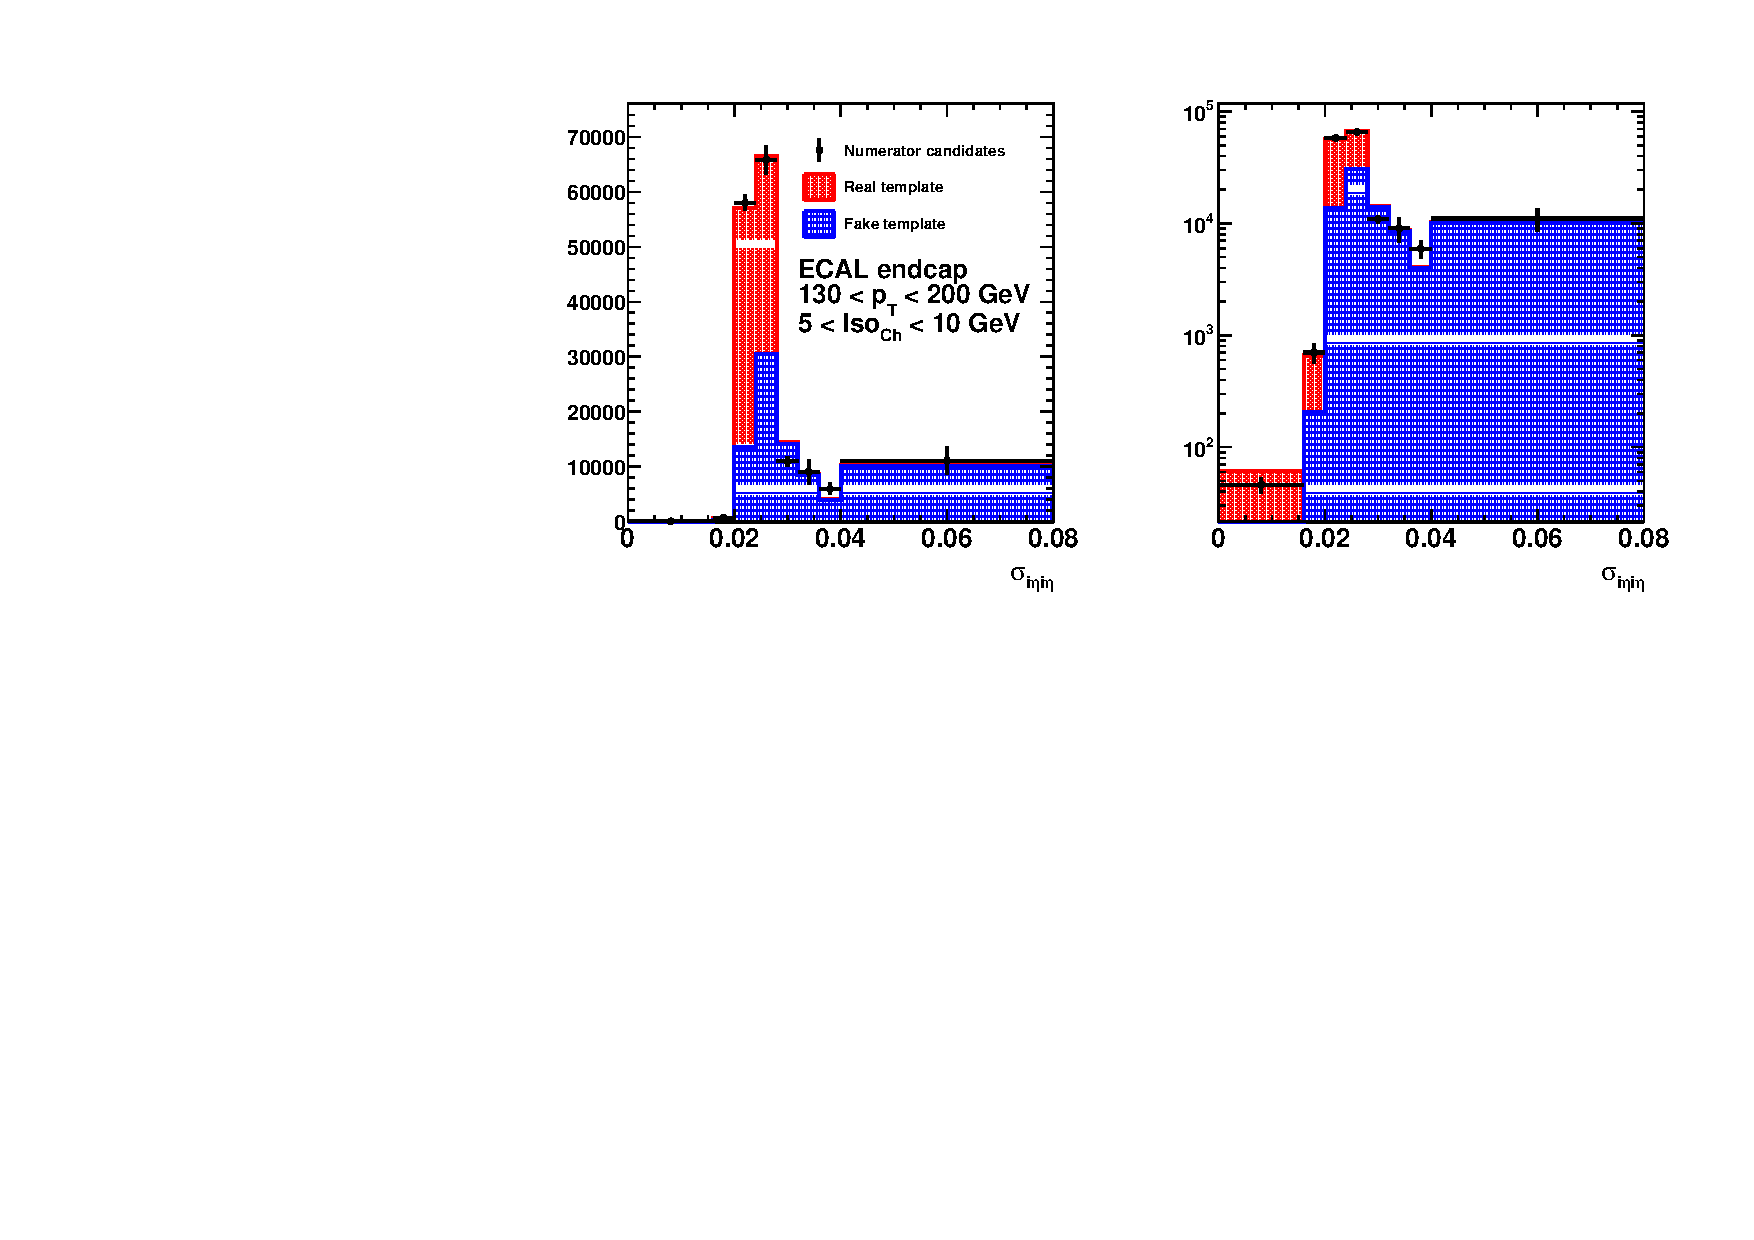
\includegraphics[scale=0.41]{figures/closure_test_h_pt130To200_chIso5To10_EE_Fake_sieie.pdf} \\
		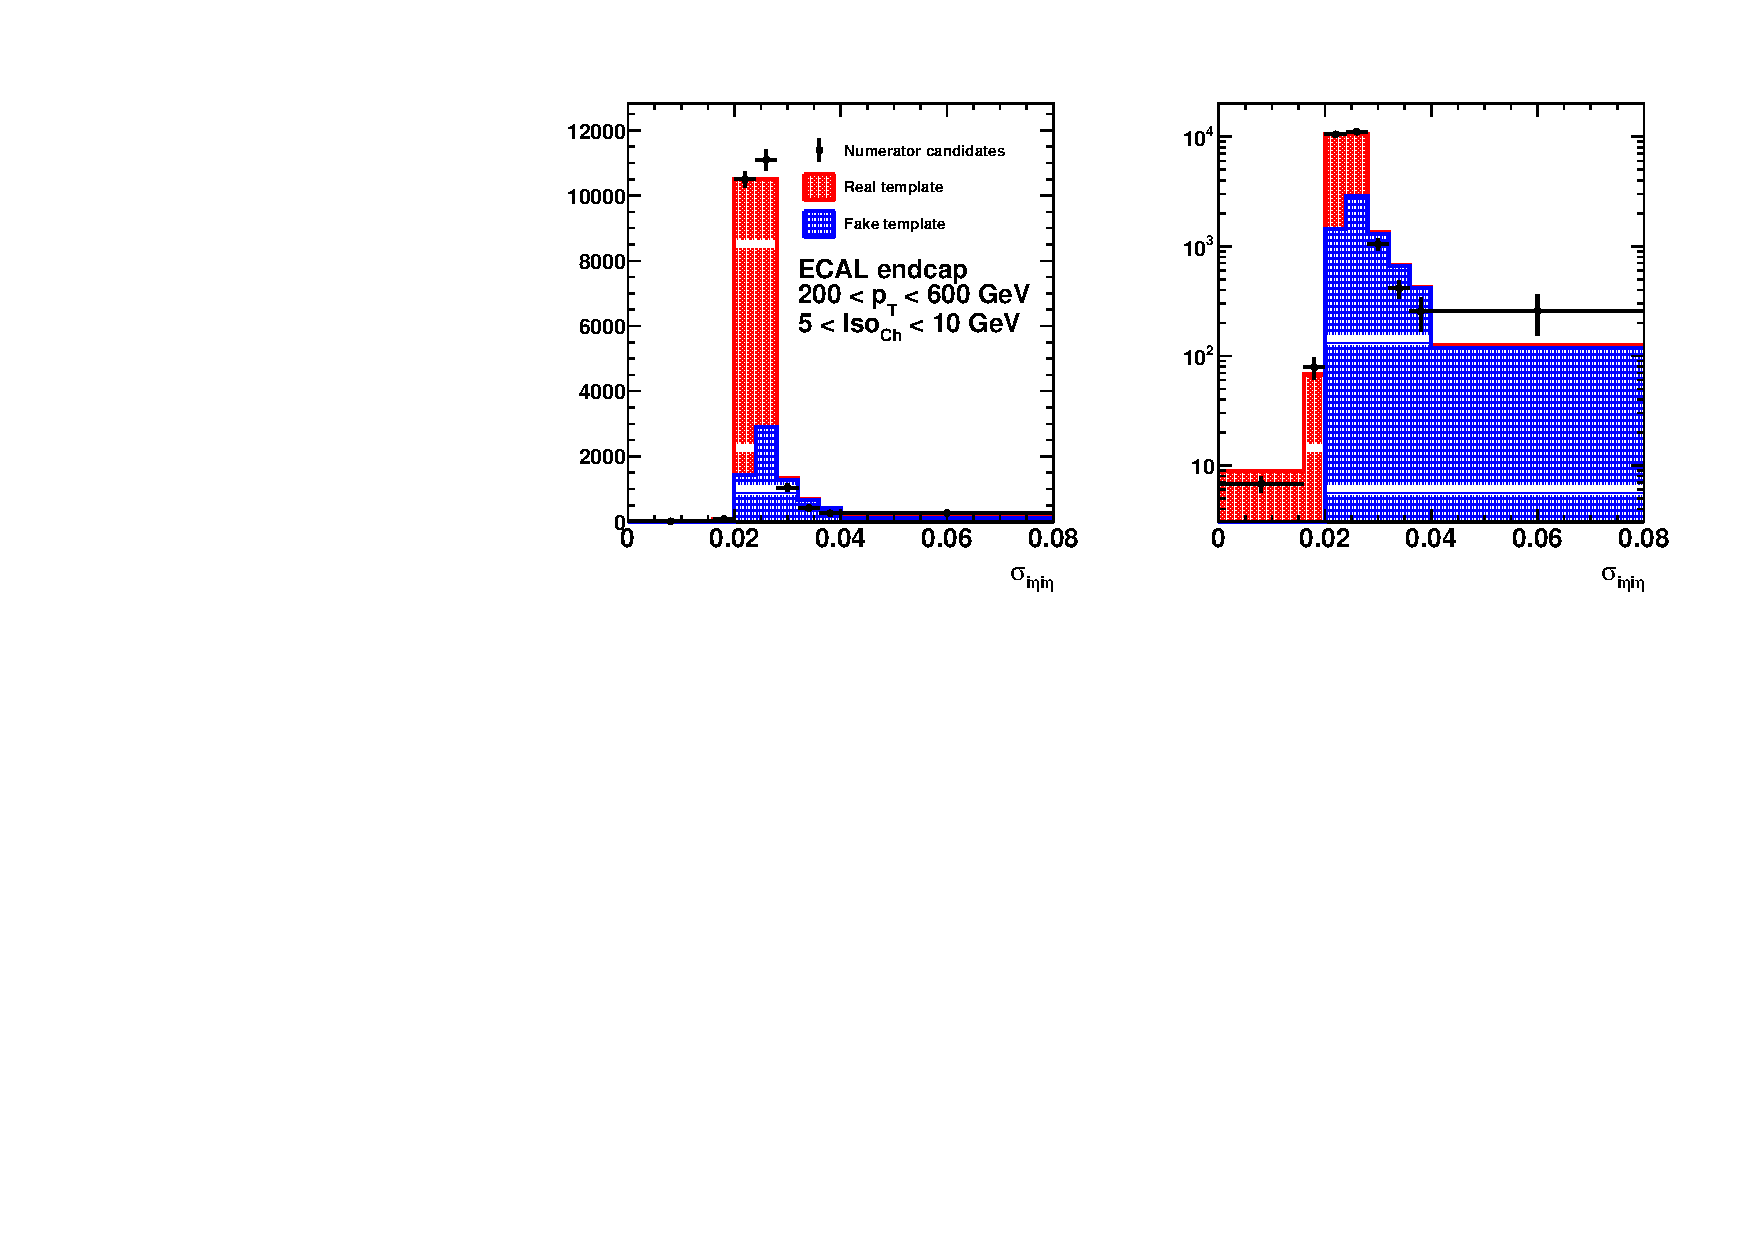
\includegraphics[scale=0.41]{figures/closure_test_h_pt200To600_chIso5To10_EE_Fake_sieie.pdf} \\
    \end{multicols}
    \vspace{-0.5cm} % temp fix for removing extra white space
  	\caption{Template fits for the MC closure test using the \sieie template variable, shown in linear and log scales, for the EB (left) and EE (right) regions. The different \pt bins are shown in the rows.}
  	\label{fig:all_mc_sieie_fits}
\end{figure}

\begin{figure}[!htbp]
	\noindent
  	\centering
  	\begin{multicols}{2}
		\includegraphics[scale=0.41]{figures/{closure_test_h_pt50To70_sieie0.0105To0.0150_EB_Fake_chIso}.pdf} \\
		\includegraphics[scale=0.41]{figures/{closure_test_h_pt70To90_sieie0.0105To0.0150_EB_Fake_chIso}.pdf} \\
		\includegraphics[scale=0.41]{figures/{closure_test_h_pt90To130_sieie0.0105To0.0150_EB_Fake_chIso}.pdf} \\
		\includegraphics[scale=0.41]{figures/{closure_test_h_pt130To200_sieie0.0105To0.0150_EB_Fake_chIso}.pdf} \\
		\includegraphics[scale=0.41]{figures/{closure_test_h_pt200To600_sieie0.0105To0.0150_EB_Fake_chIso}.pdf} \\
		\includegraphics[scale=0.41]{figures/{closure_test_h_pt50To70_sieie0.0280To0.0400_EE_Fake_chIso}.pdf} \\
		\includegraphics[scale=0.41]{figures/{closure_test_h_pt70To90_sieie0.0280To0.0400_EE_Fake_chIso}.pdf} \\
		\includegraphics[scale=0.41]{figures/{closure_test_h_pt90To130_sieie0.0280To0.0400_EE_Fake_chIso}.pdf} \\
		\includegraphics[scale=0.41]{figures/{closure_test_h_pt130To200_sieie0.0280To0.0400_EE_Fake_chIso}.pdf} \\
		\includegraphics[scale=0.41]{figures/{closure_test_h_pt200To600_sieie0.0280To0.0400_EE_Fake_chIso}.pdf} \\
	\end{multicols}
	\vspace{-0.5cm} % temp fix for removing extra white space
  	\caption{Template fits for the MC closure test using the \chiso template variable, shown in linear and log scales, for the EB (left) and EE (right) regions. The different \pt bins are shown in the rows.}
  	\label{fig:all_mc_chiso_fits}
\end{figure}

\pagebreak

\section{The MC Fake Templates}\label{sec:mc_fake_templates}

The fake templates in \sieie used in the MC based closure test to the photon fake rate method are shown in Fig.~\ref{fig:all_mc_sieie_fake_templates} for the EB and EE categories. The templates are shown in \pt bins of 50-70, 70-90, 90-130, 130-200, and 200-600\GeV. For each \pt bin, the templates constructed using the nominal \chiso sideband of 5-10\GeV are compared to those derived using the MC truth information, which can be considered the ideal fake template corresponding in that \pt bin. The fake templates in \chiso using these same \pt bins are shown in Fig.~\ref{fig:all_mc_chiso_fake_templates} for the EB and EE categories. The templates constructed using different \sieie sidebands are compared against the fake templates derived using the MC truth information in the simulated sample for the EB and EE categories.

\begin{figure}[!htbp]
	\noindent
	\centering
	\begin{multicols}{2}
		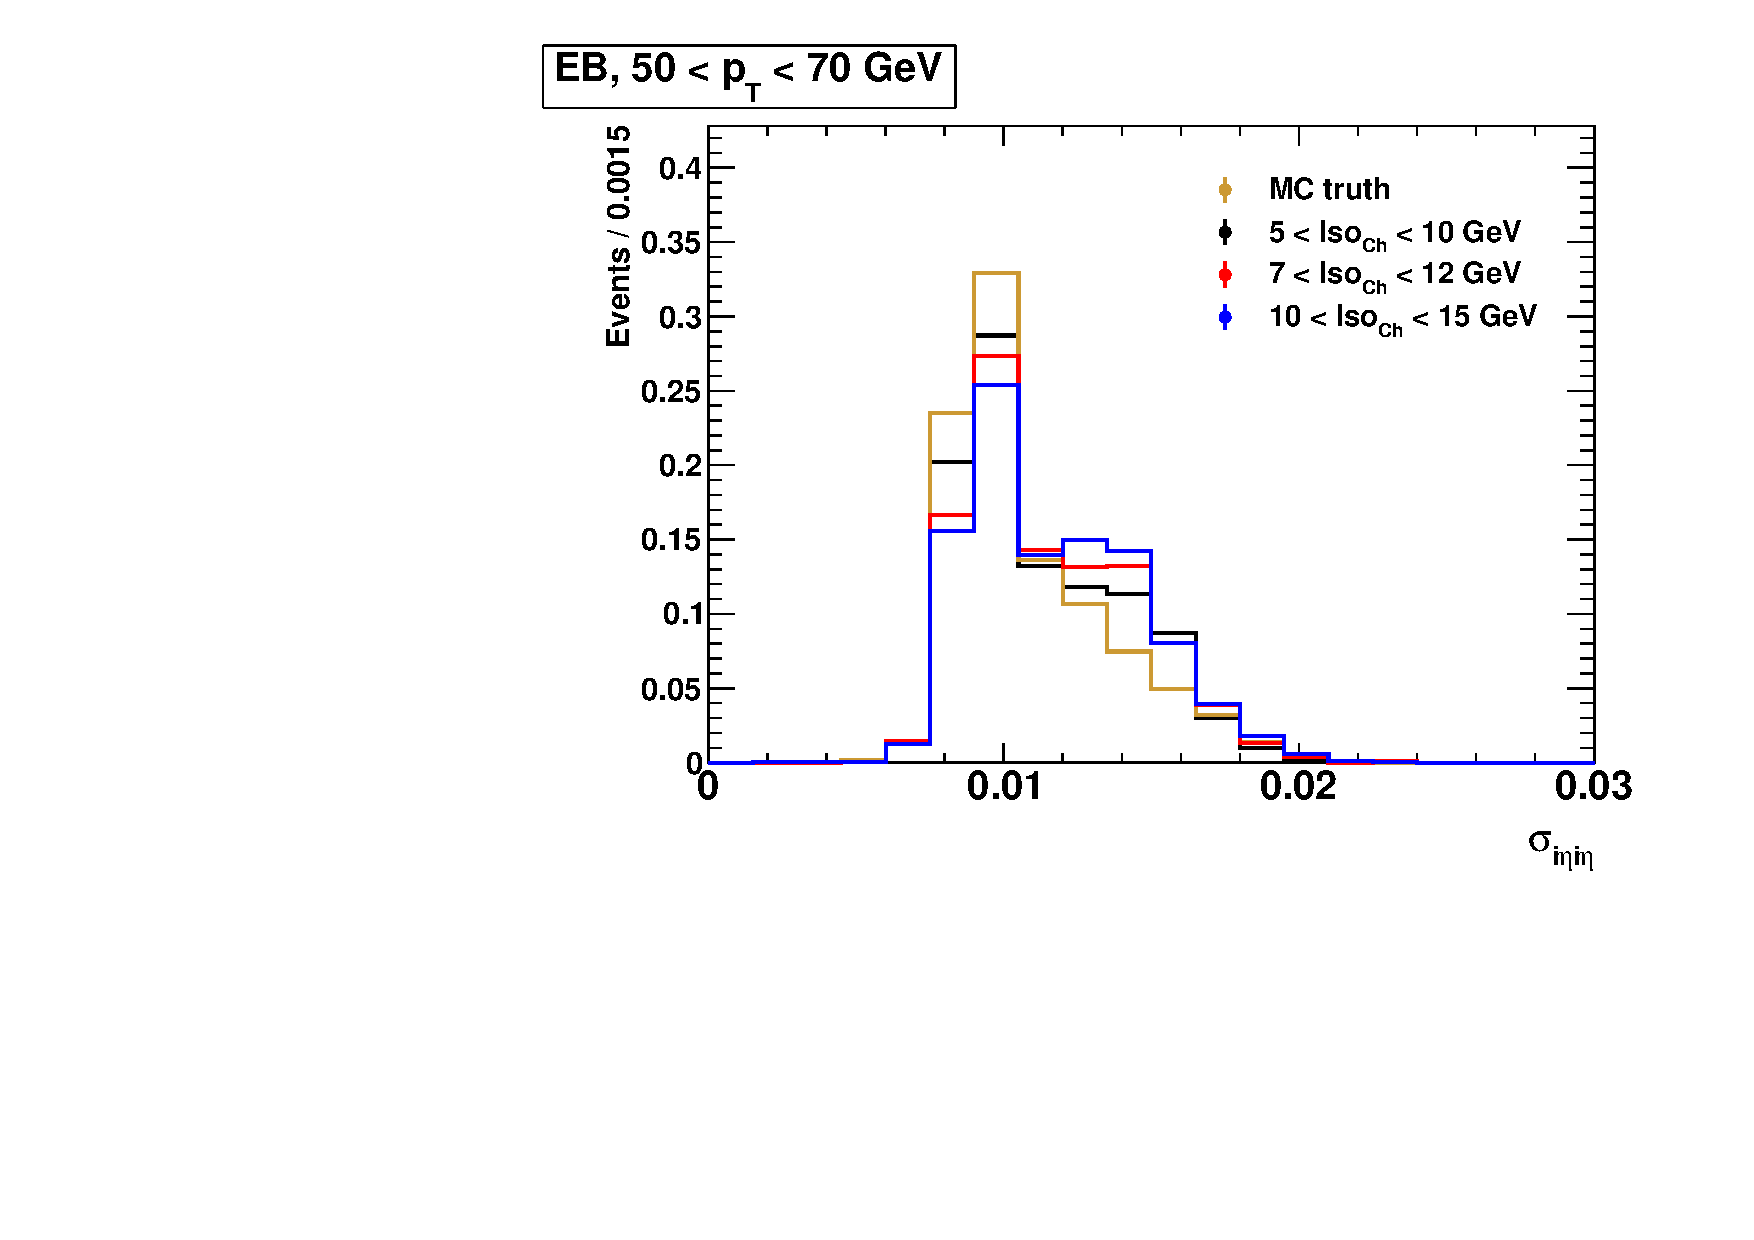
\includegraphics[scale=0.29]{figures/closure_test_fake_template_sieie_EB_pt50To70_sample_all.pdf} \\
		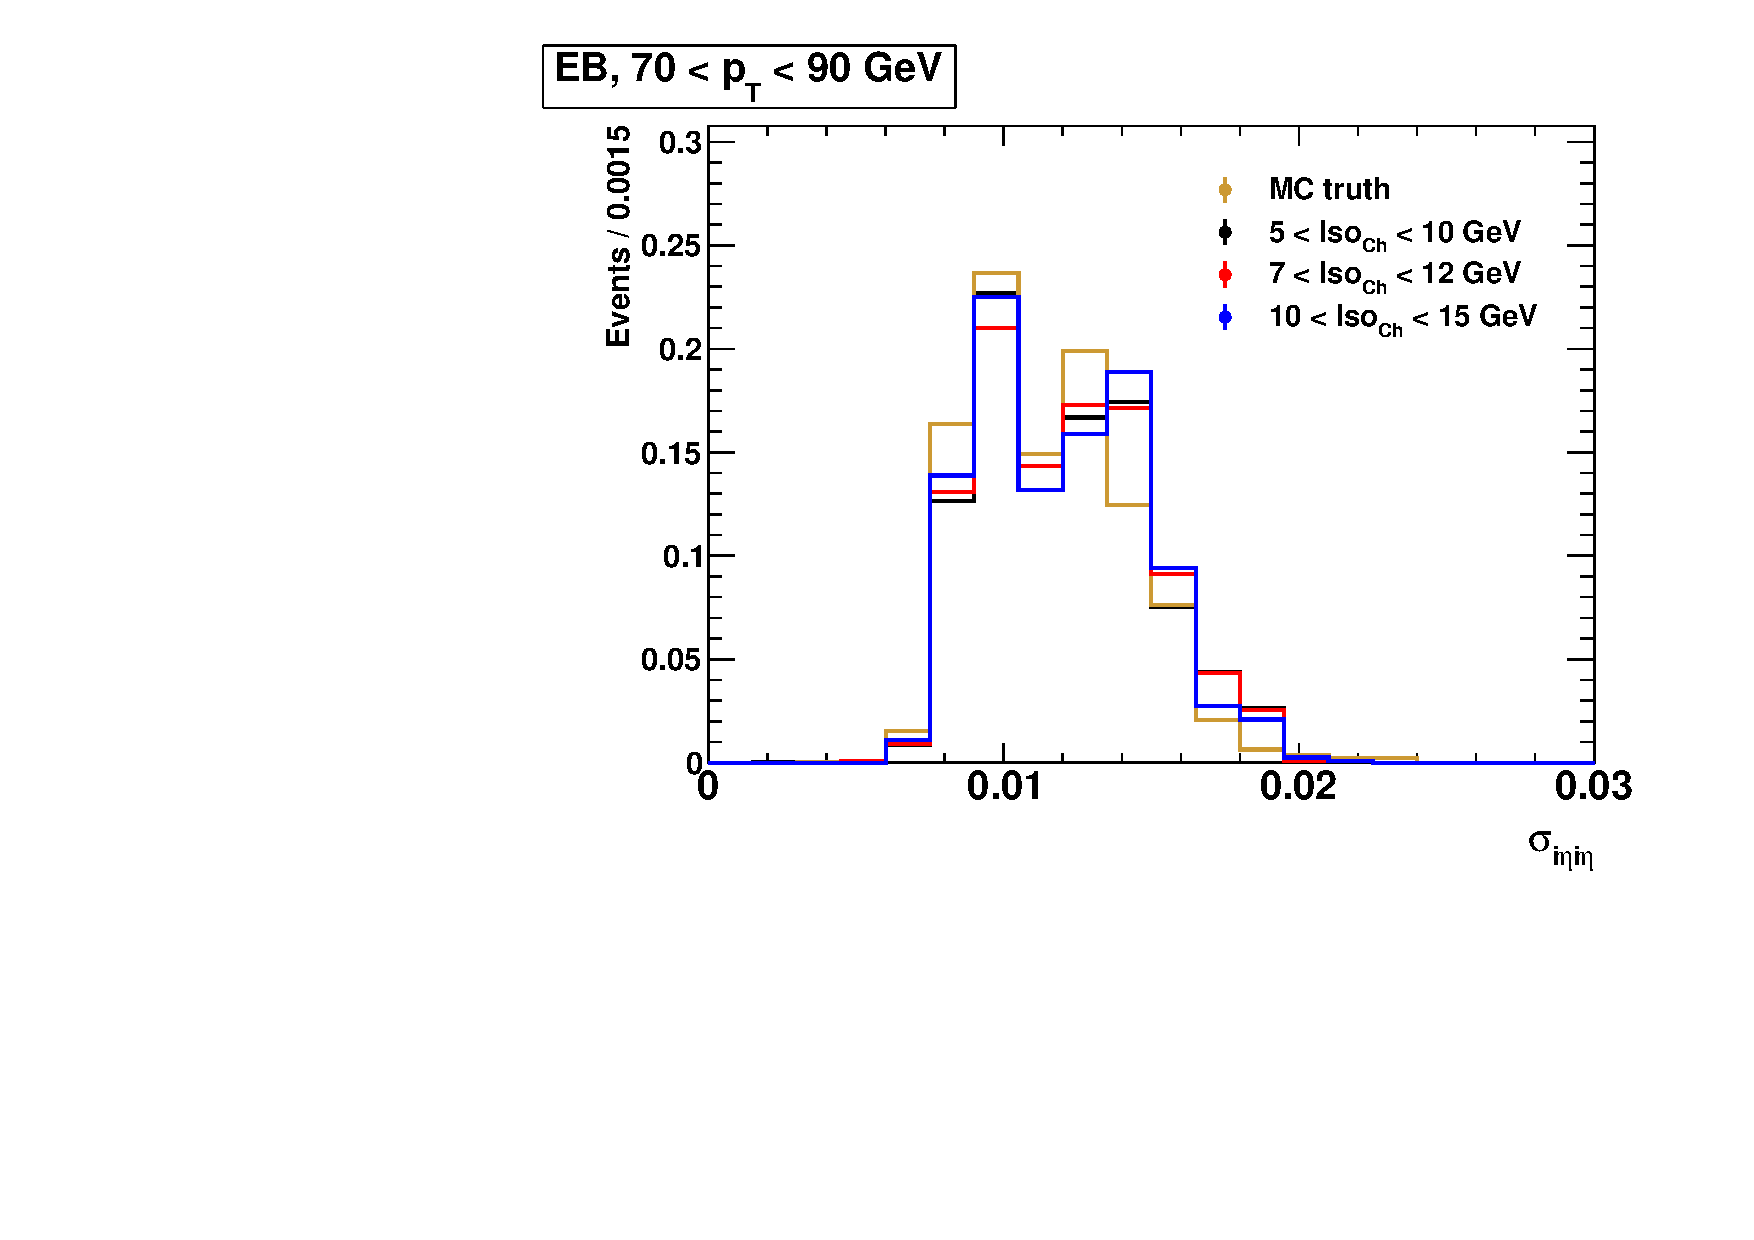
\includegraphics[scale=0.29]{figures/closure_test_fake_template_sieie_EB_pt70To90_sample_all.pdf} \\
		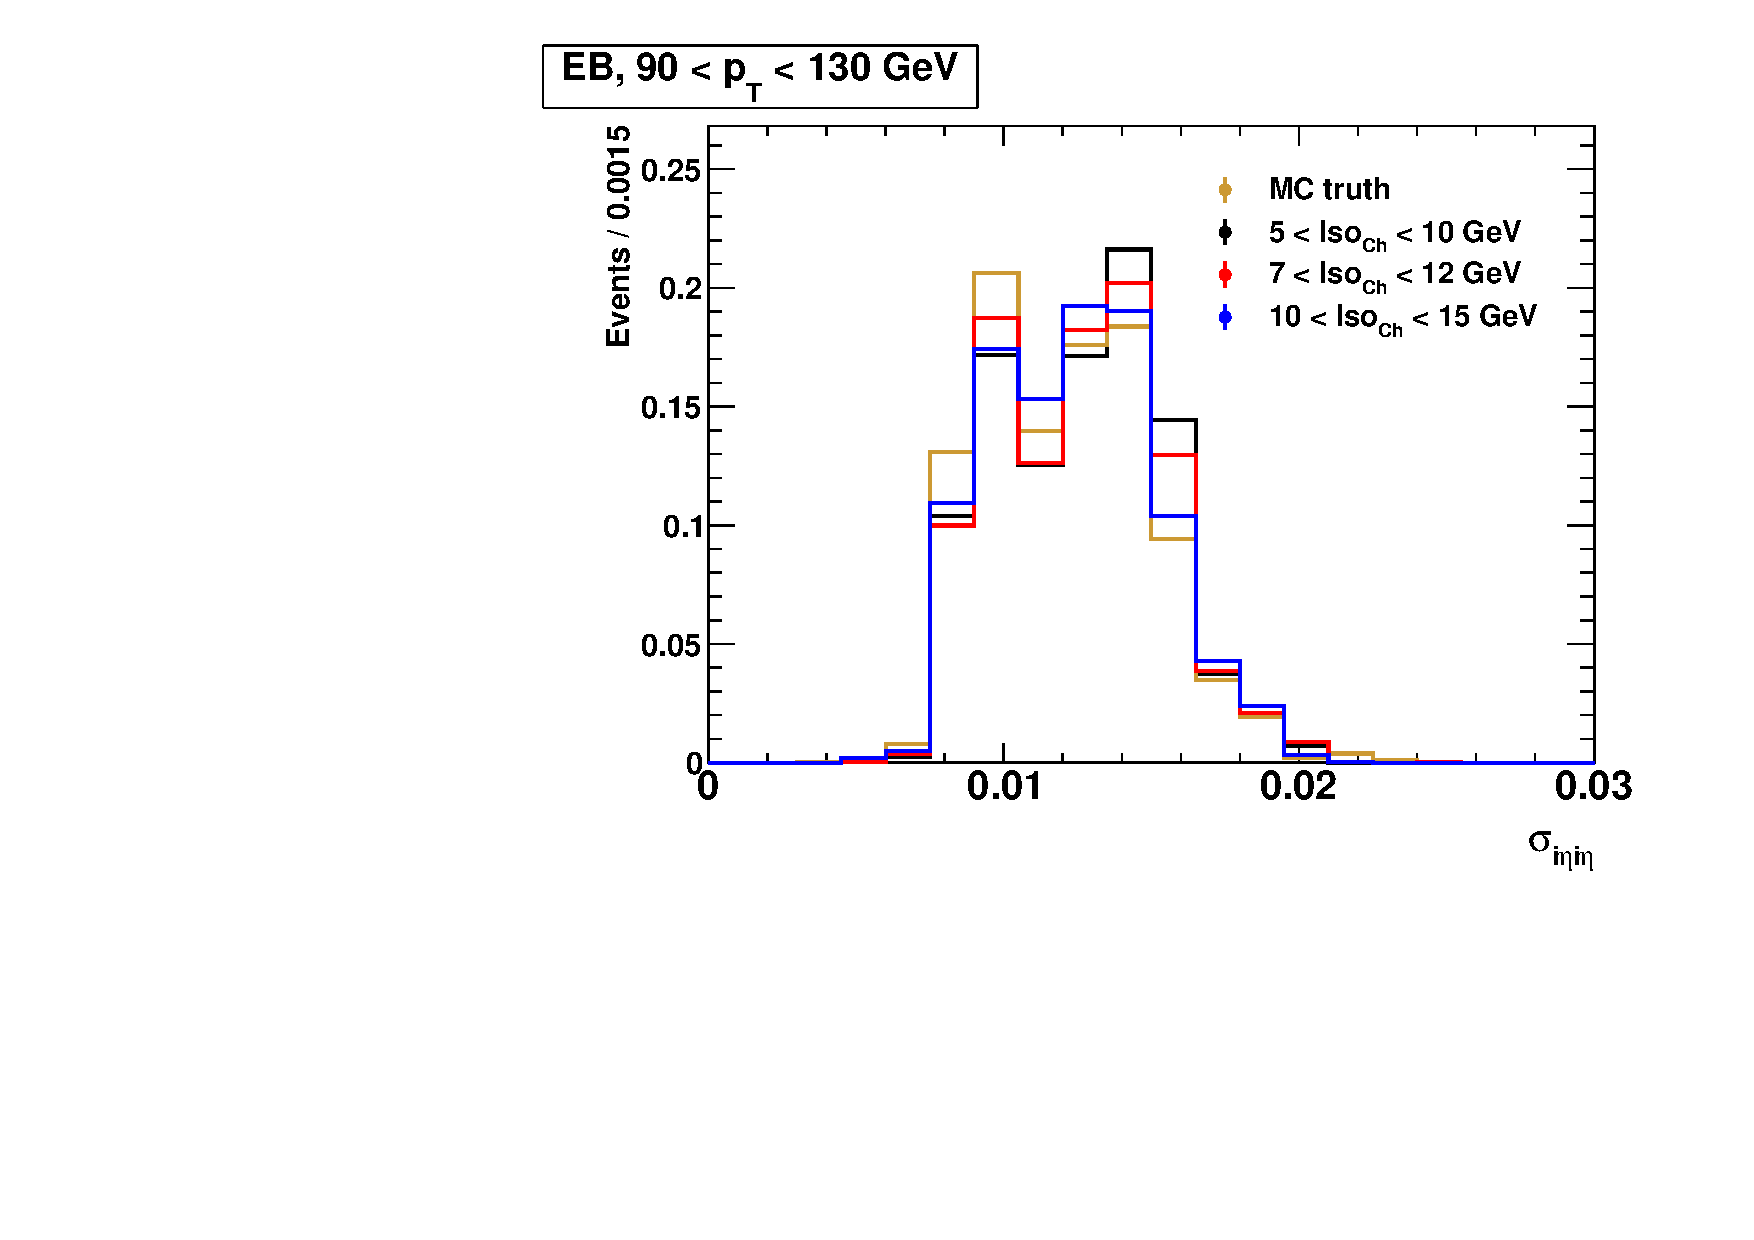
\includegraphics[scale=0.29]{figures/closure_test_fake_template_sieie_EB_pt90To130_sample_all.pdf} \\
		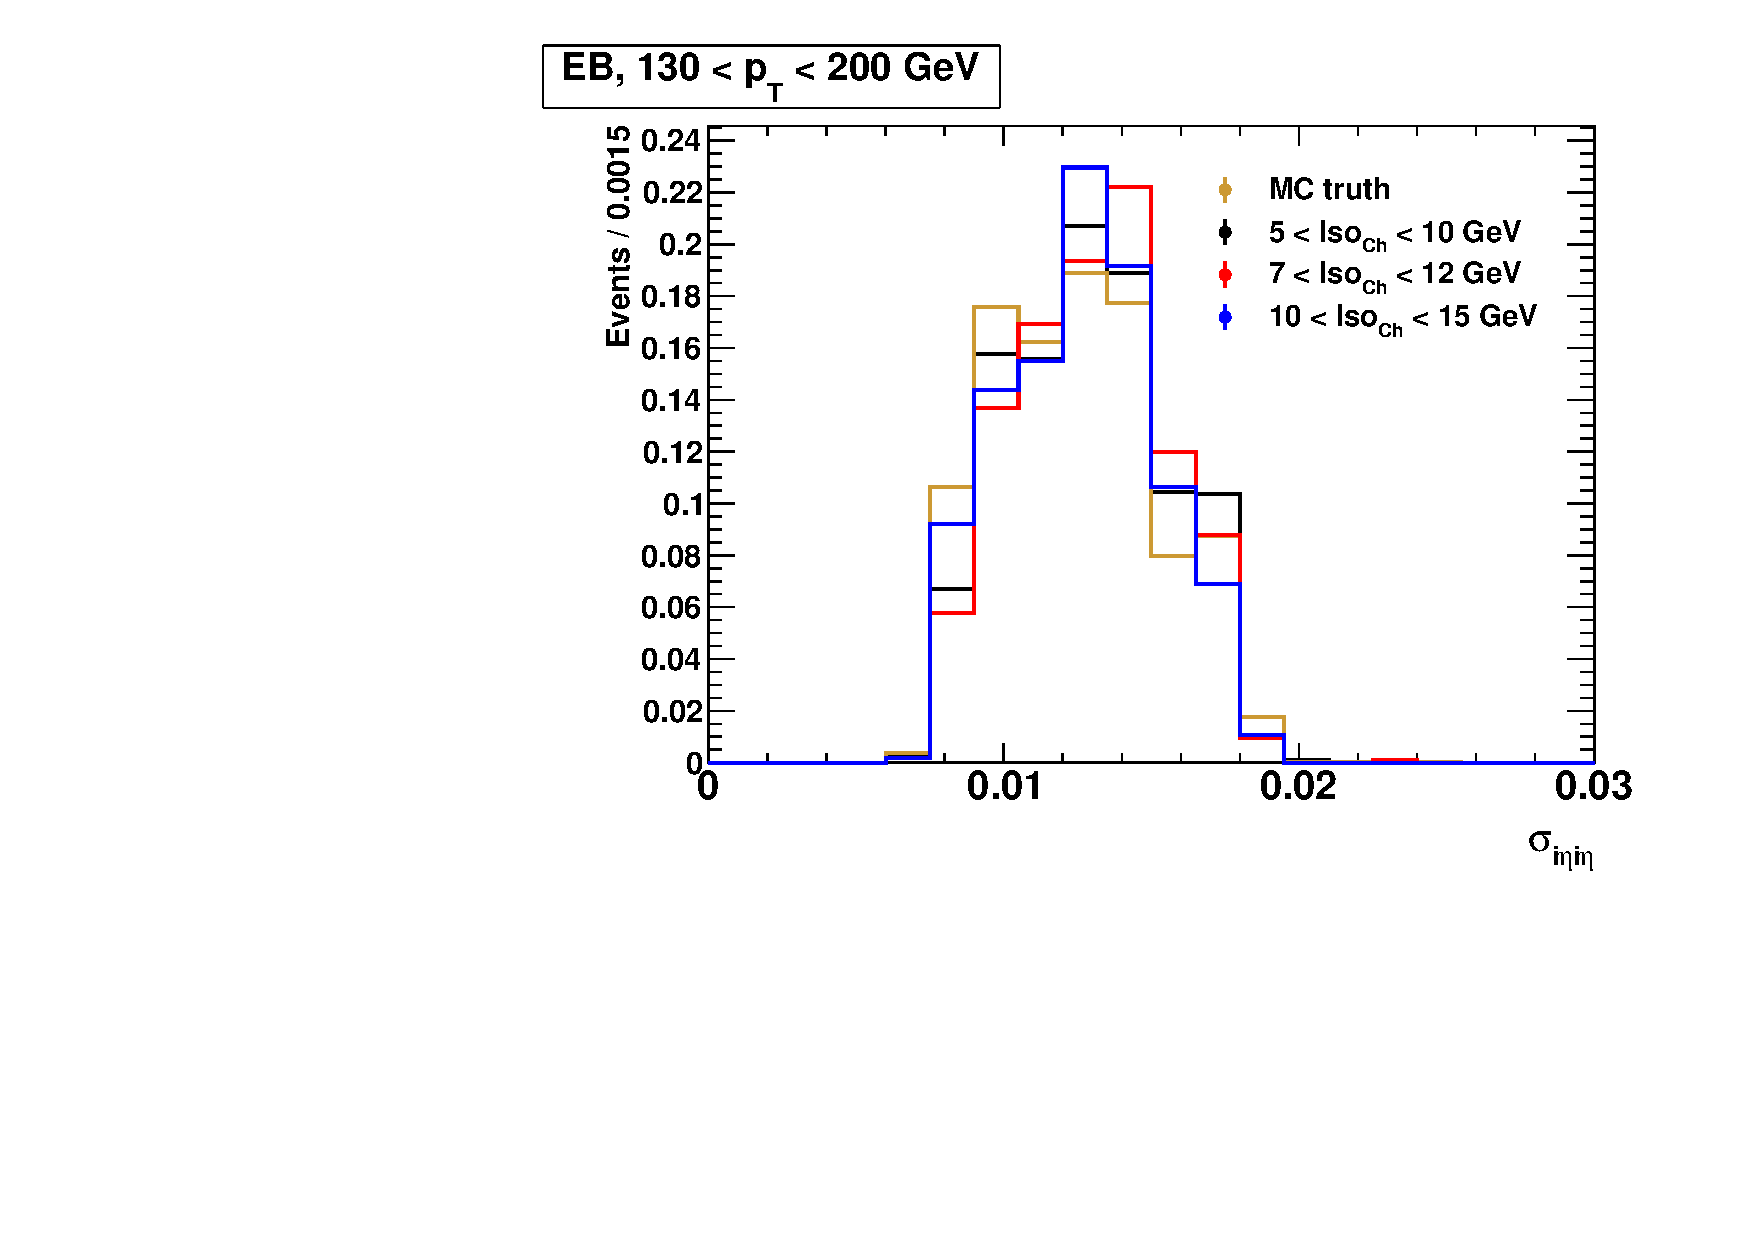
\includegraphics[scale=0.29]{figures/closure_test_fake_template_sieie_EB_pt130To200_sample_all.pdf} \\
		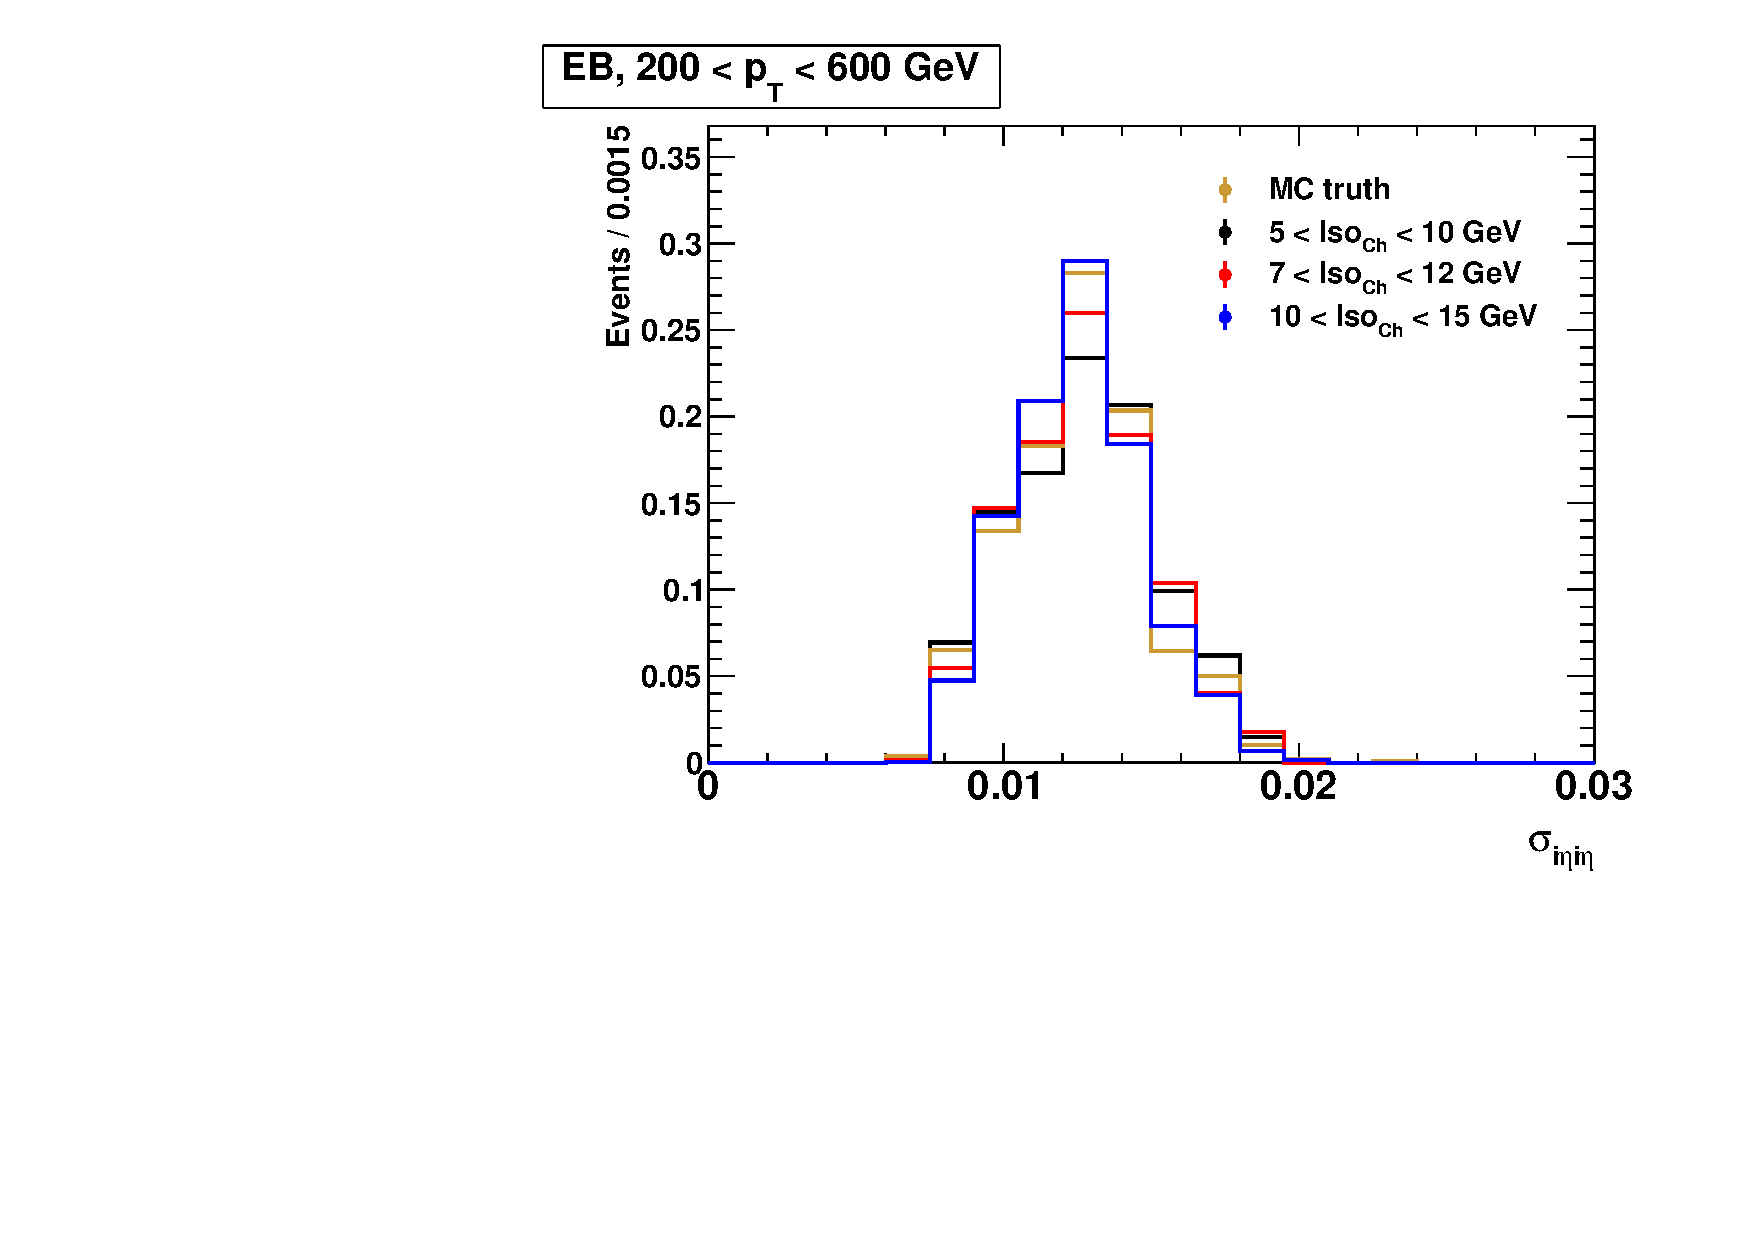
\includegraphics[scale=0.29]{figures/closure_test_fake_template_sieie_EB_pt200To600_sample_all.pdf} \\
		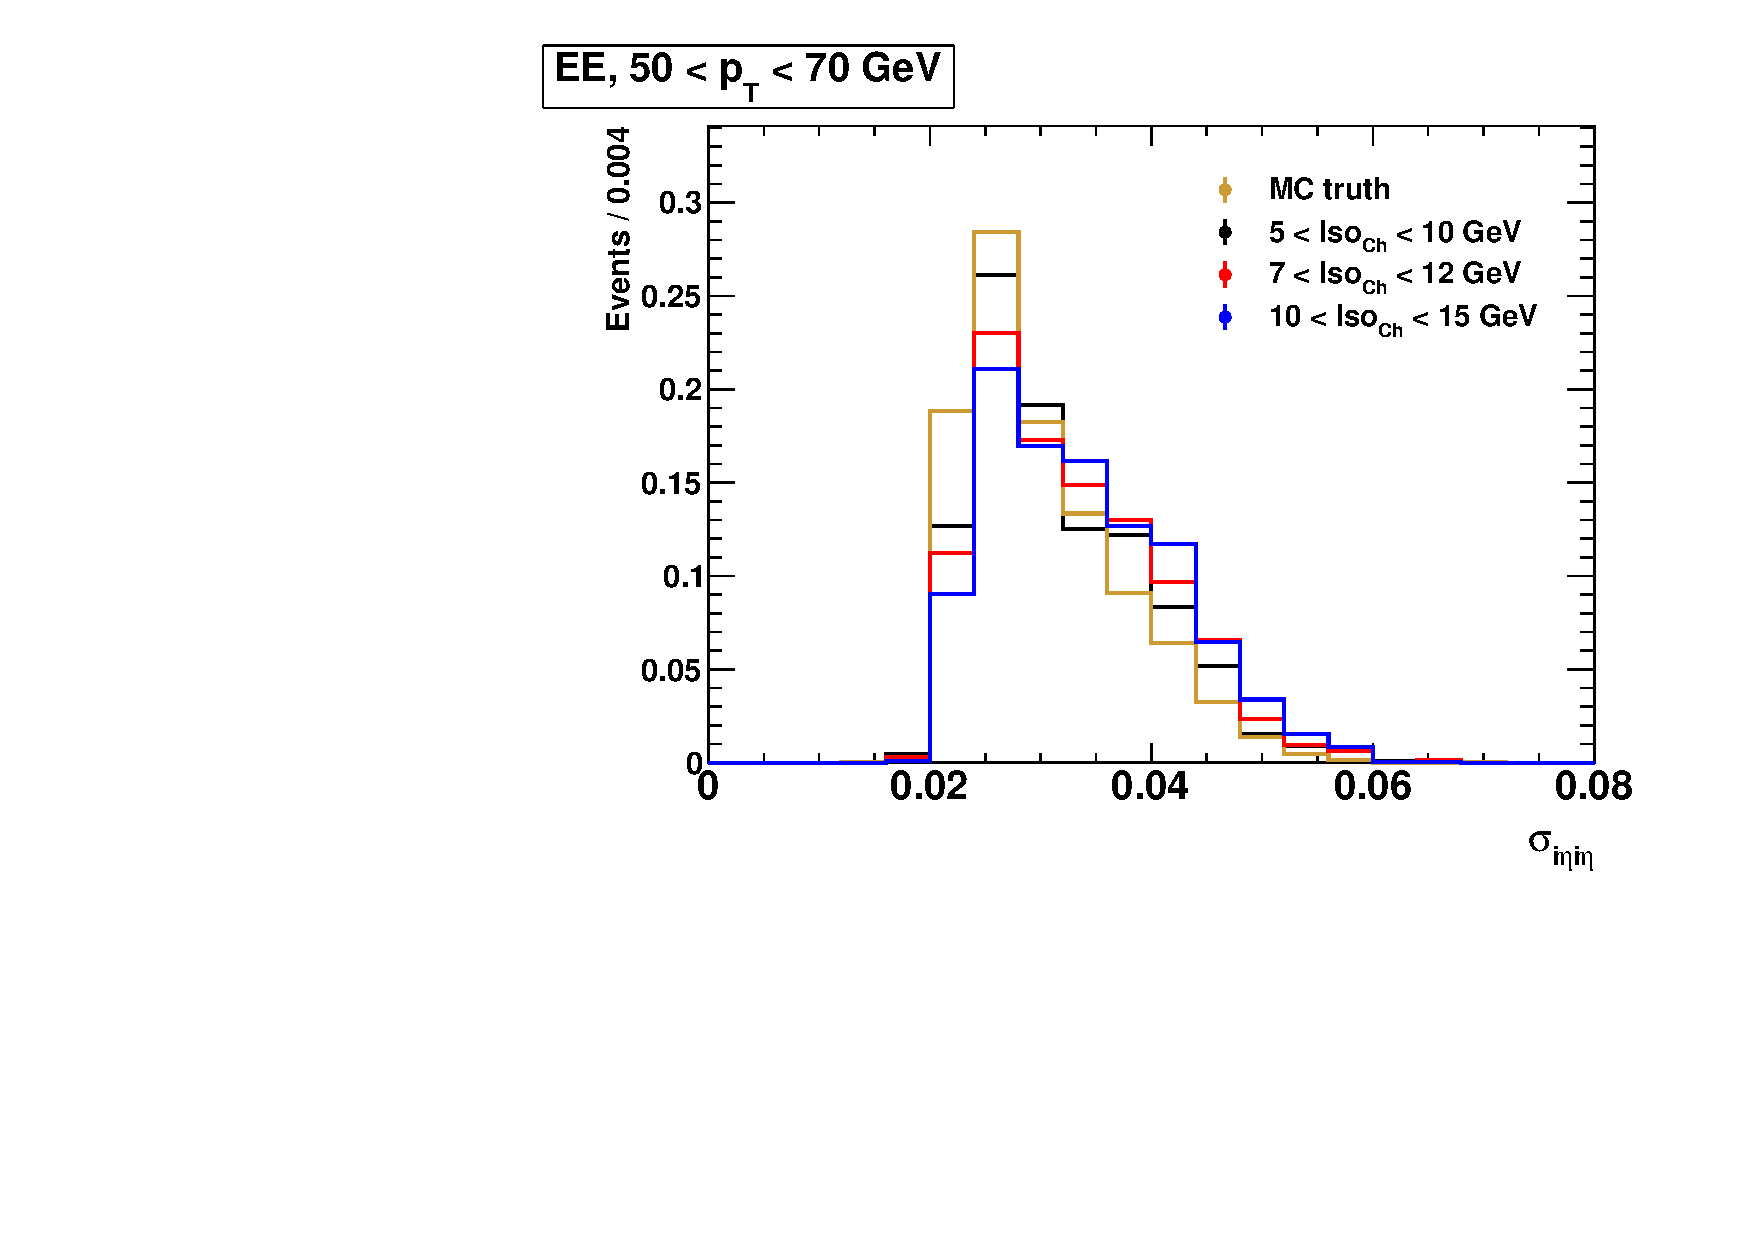
\includegraphics[scale=0.29]{figures/closure_test_fake_template_sieie_EE_pt50To70_sample_all.pdf} \\
		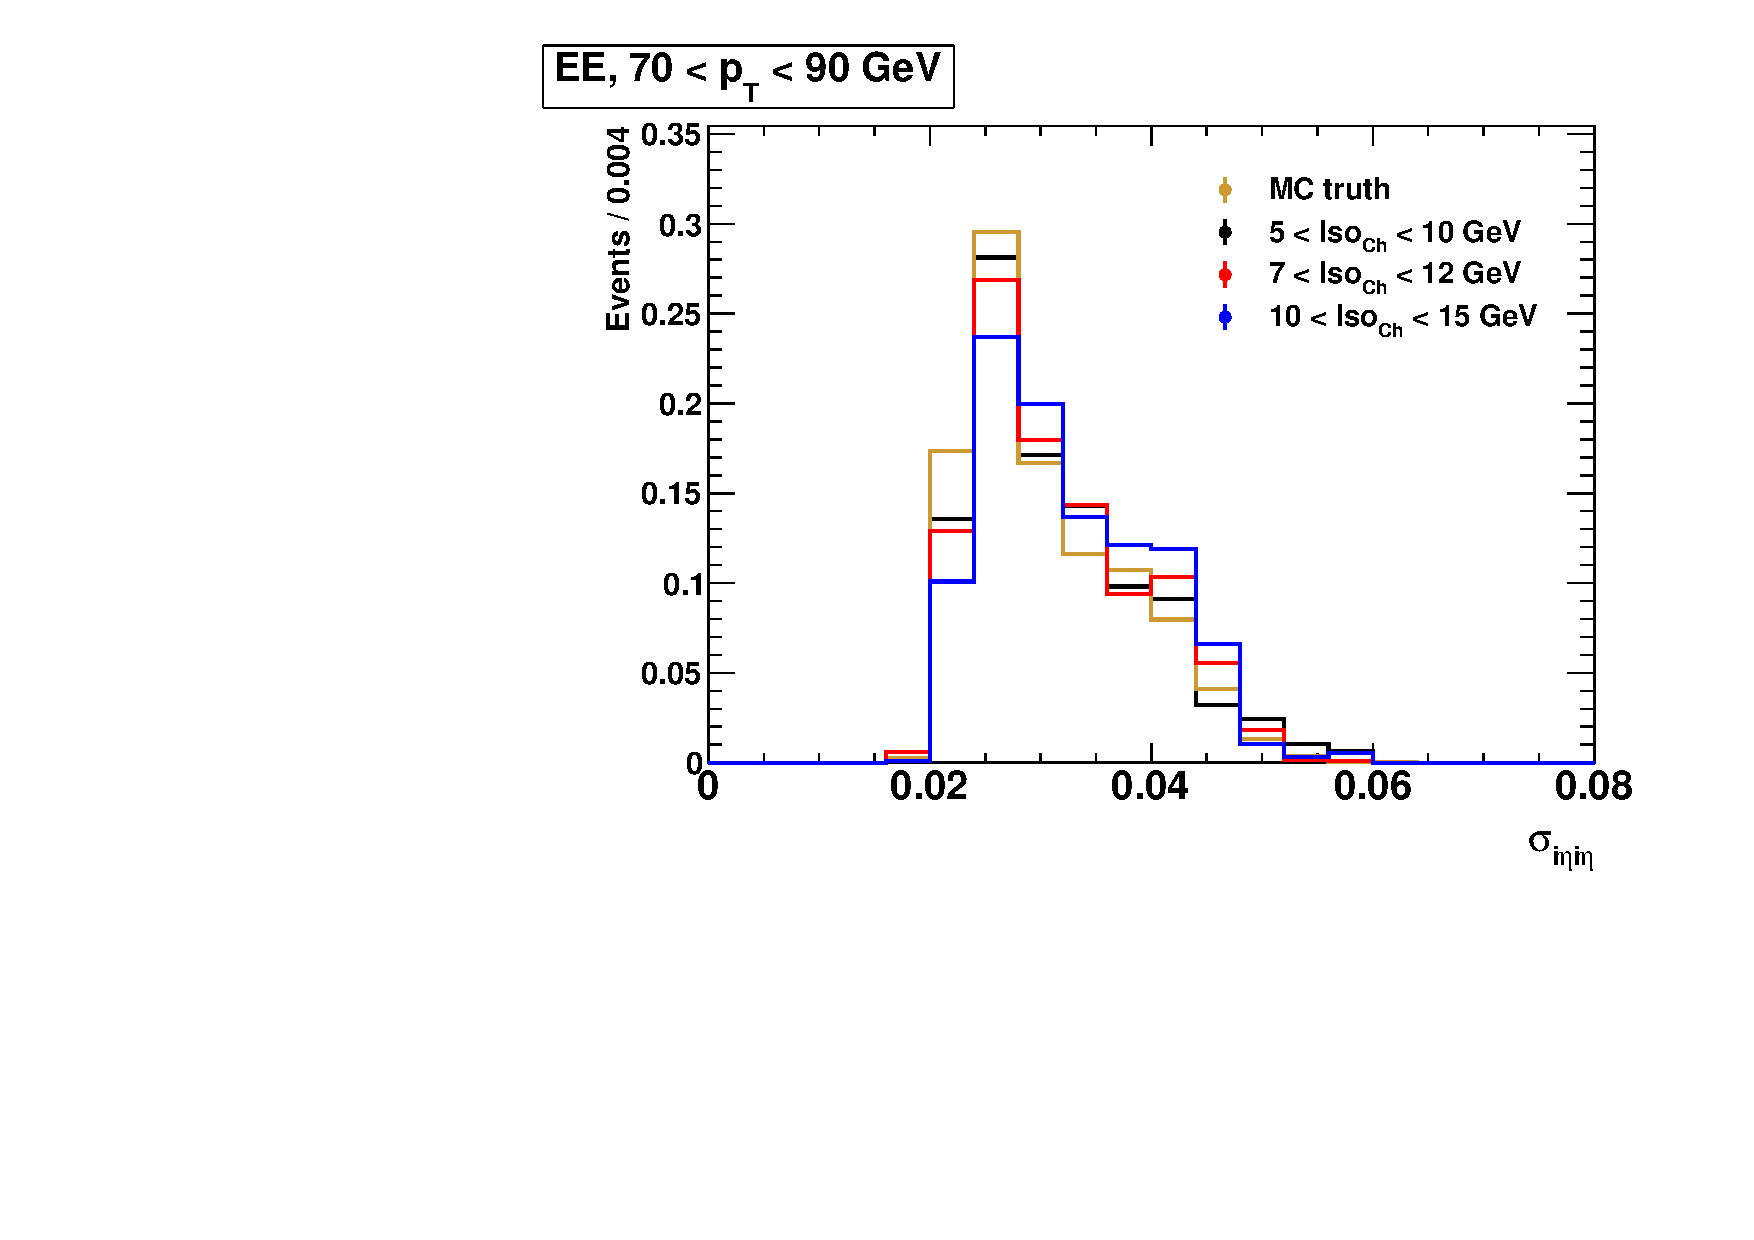
\includegraphics[scale=0.29]{figures/closure_test_fake_template_sieie_EE_pt70To90_sample_all.pdf} \\
		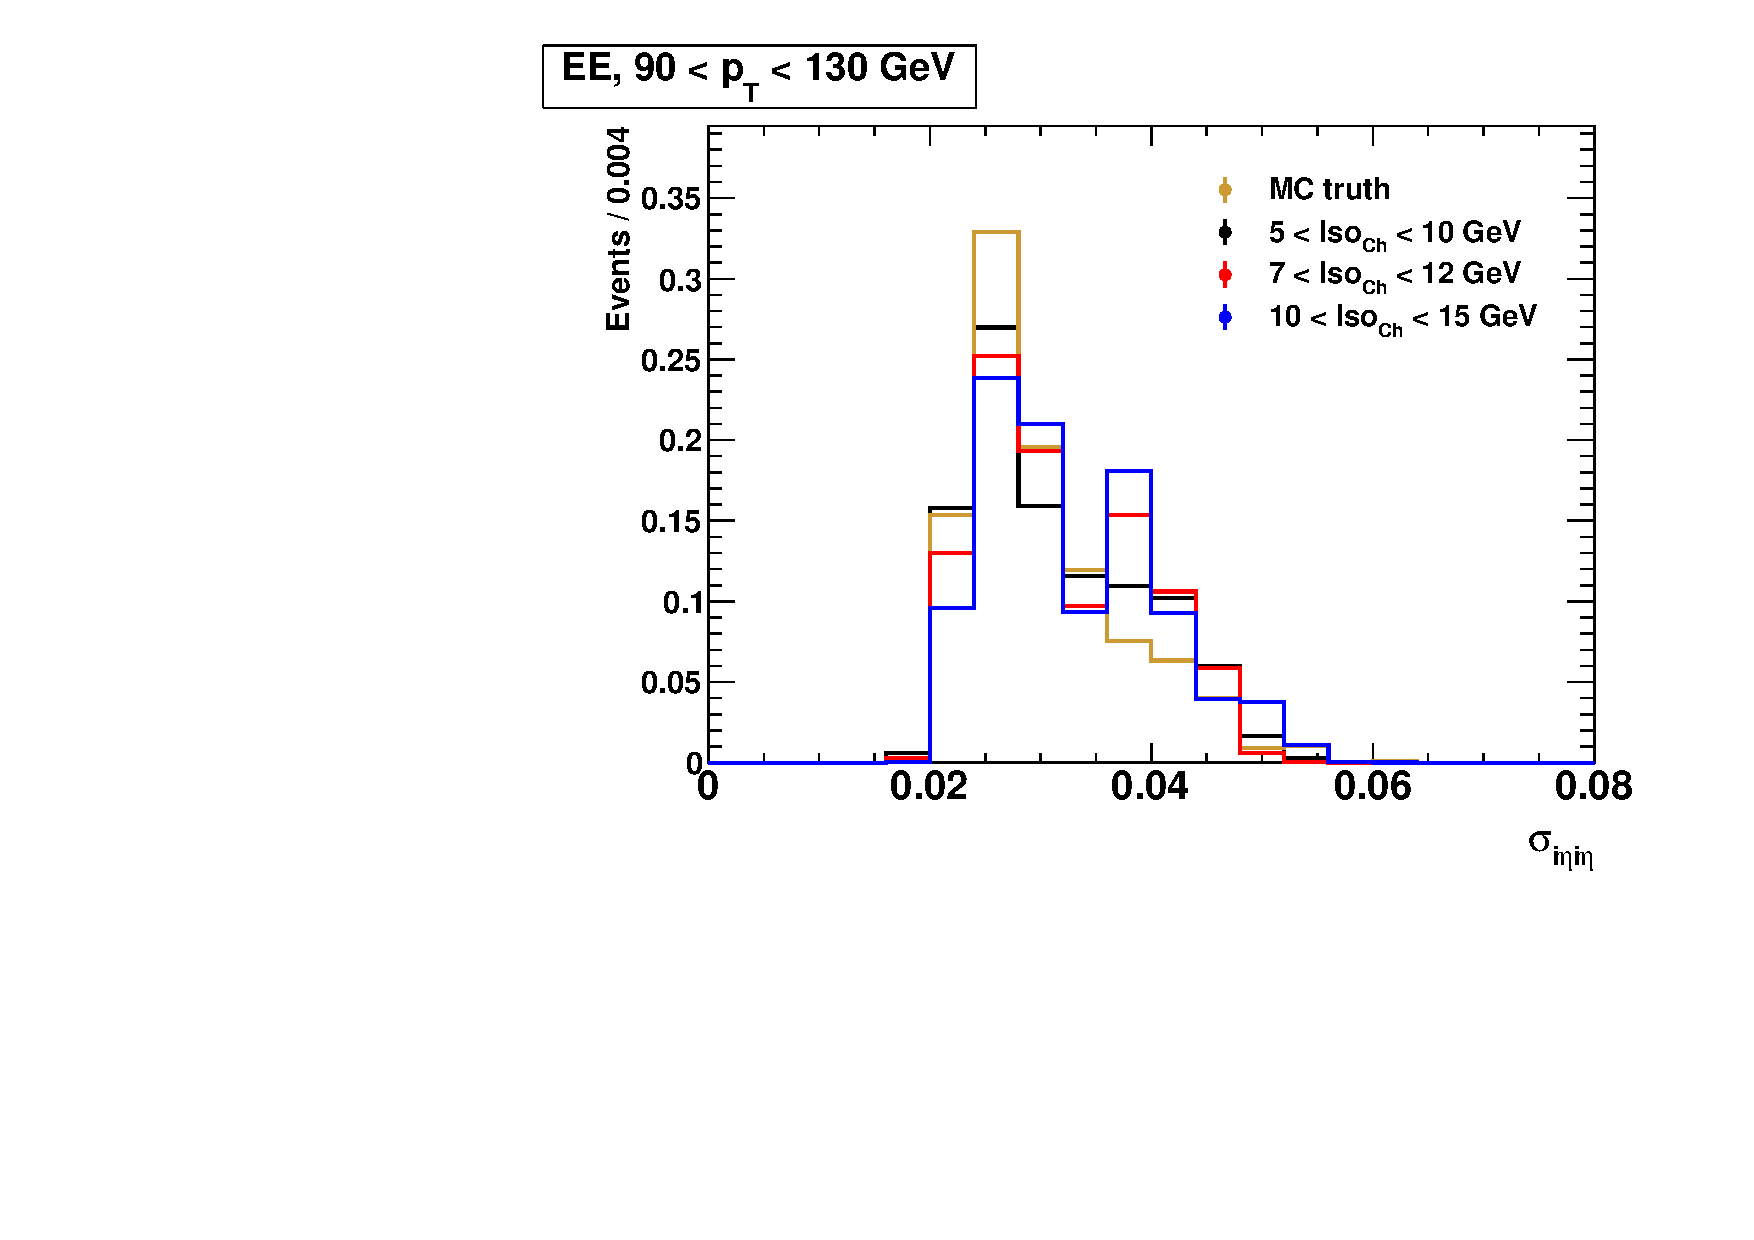
\includegraphics[scale=0.29]{figures/closure_test_fake_template_sieie_EE_pt90To130_sample_all.pdf} \\
		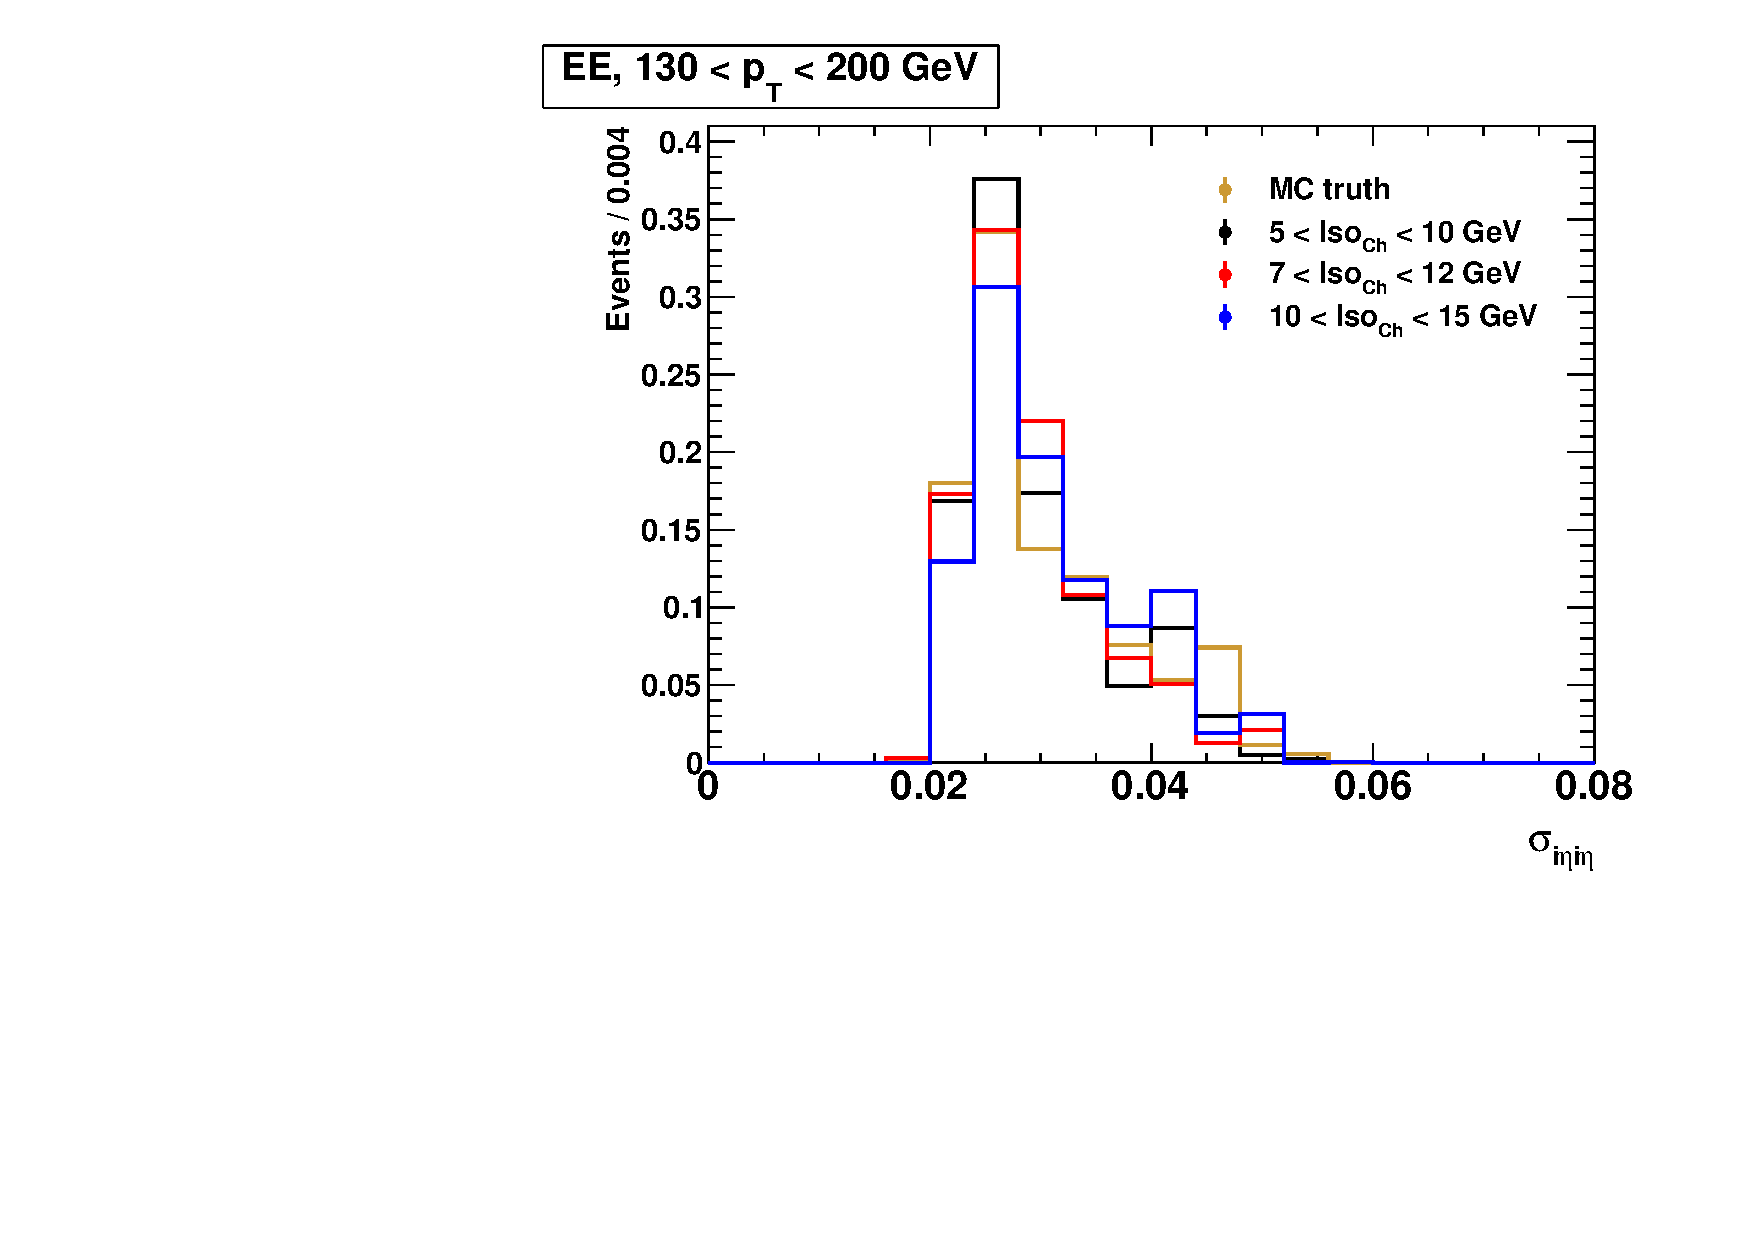
\includegraphics[scale=0.29]{figures/closure_test_fake_template_sieie_EE_pt130To200_sample_all.pdf} \\
		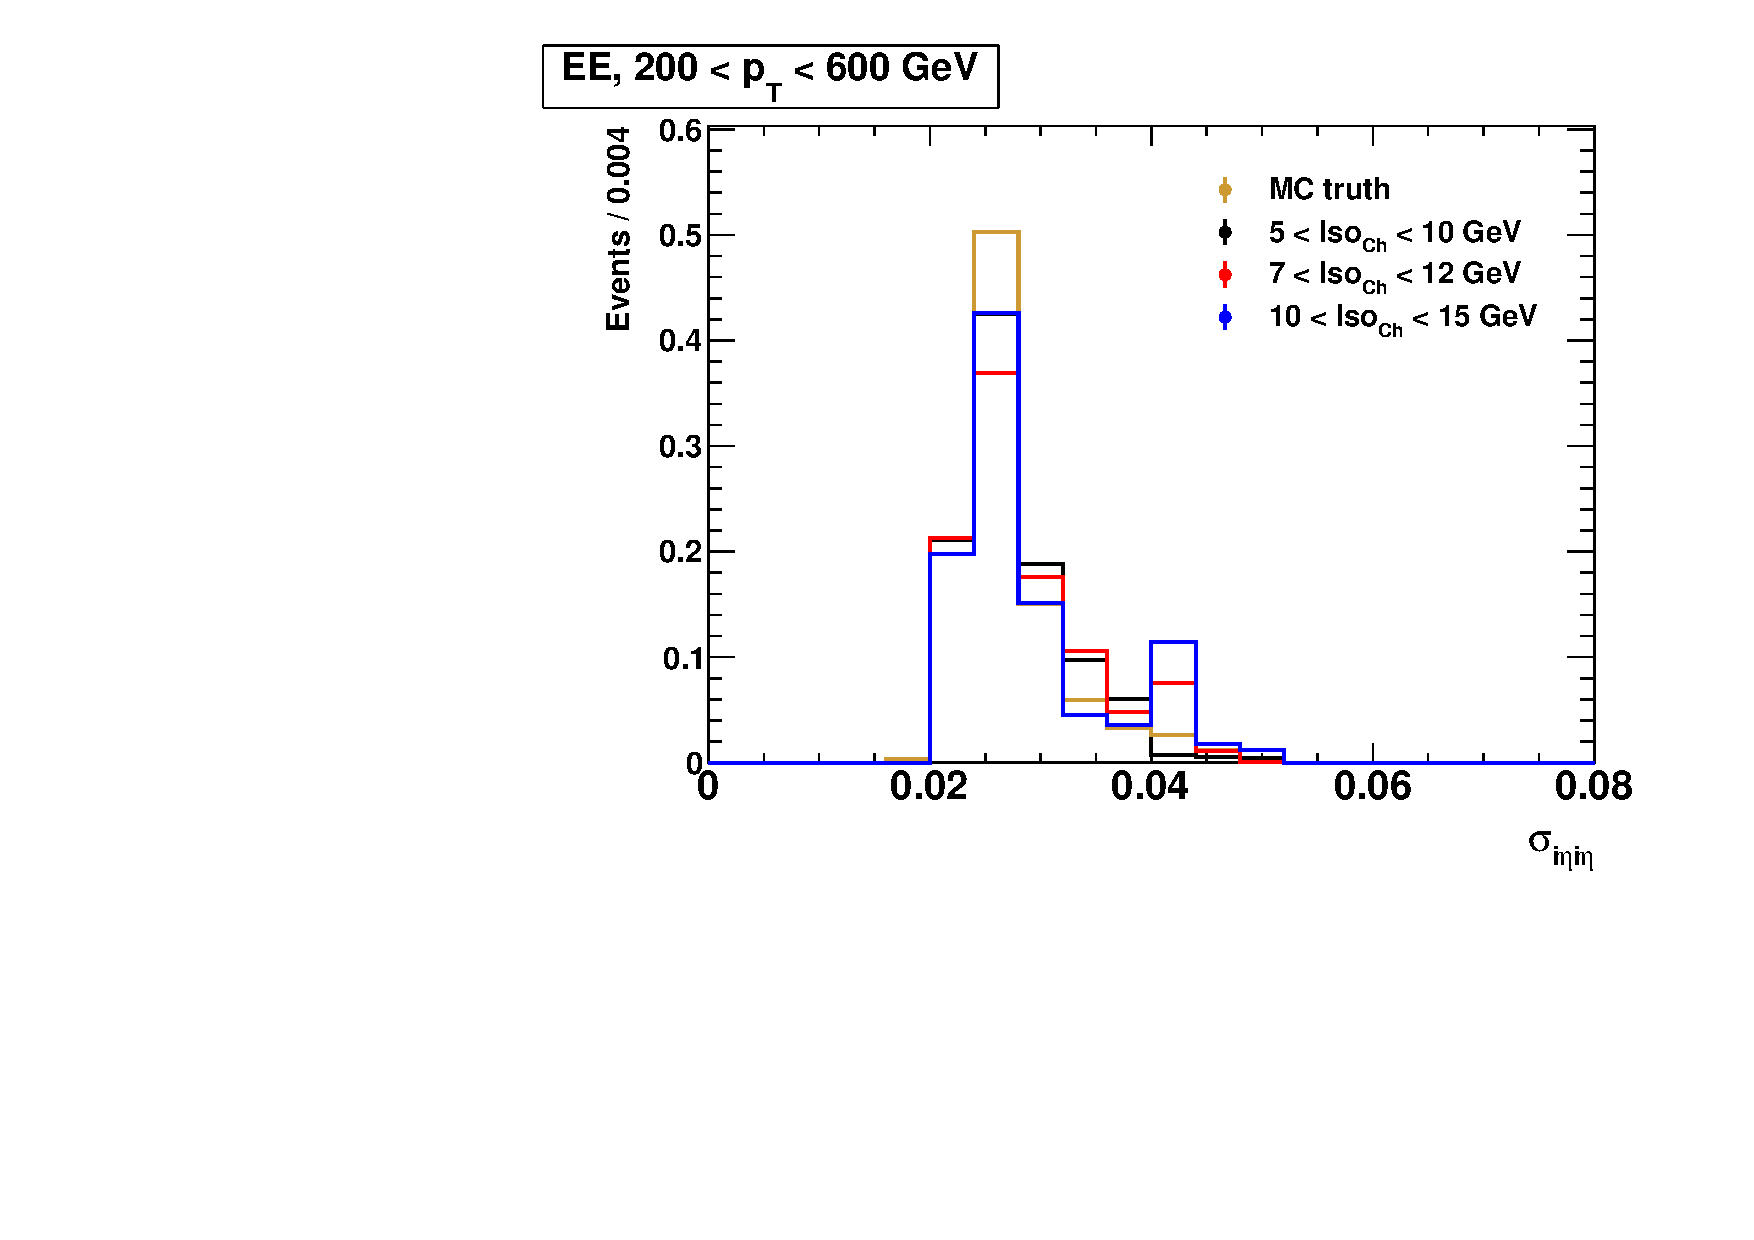
\includegraphics[scale=0.29]{figures/closure_test_fake_template_sieie_EE_pt200To600_sample_all.pdf} \\
	\end{multicols}
	\vspace{-0.5cm} % temp fix for removing extra white space
  	\caption{Fake templates in \sieie from simulation in the EB (left) and EE (right) categories for various \pt bins, shown in the rows.}
  	\label{fig:all_mc_sieie_fake_templates}
\end{figure}


\begin{figure}[!htbp]
	\noindent
	\centering
	\begin{multicols}{2}
		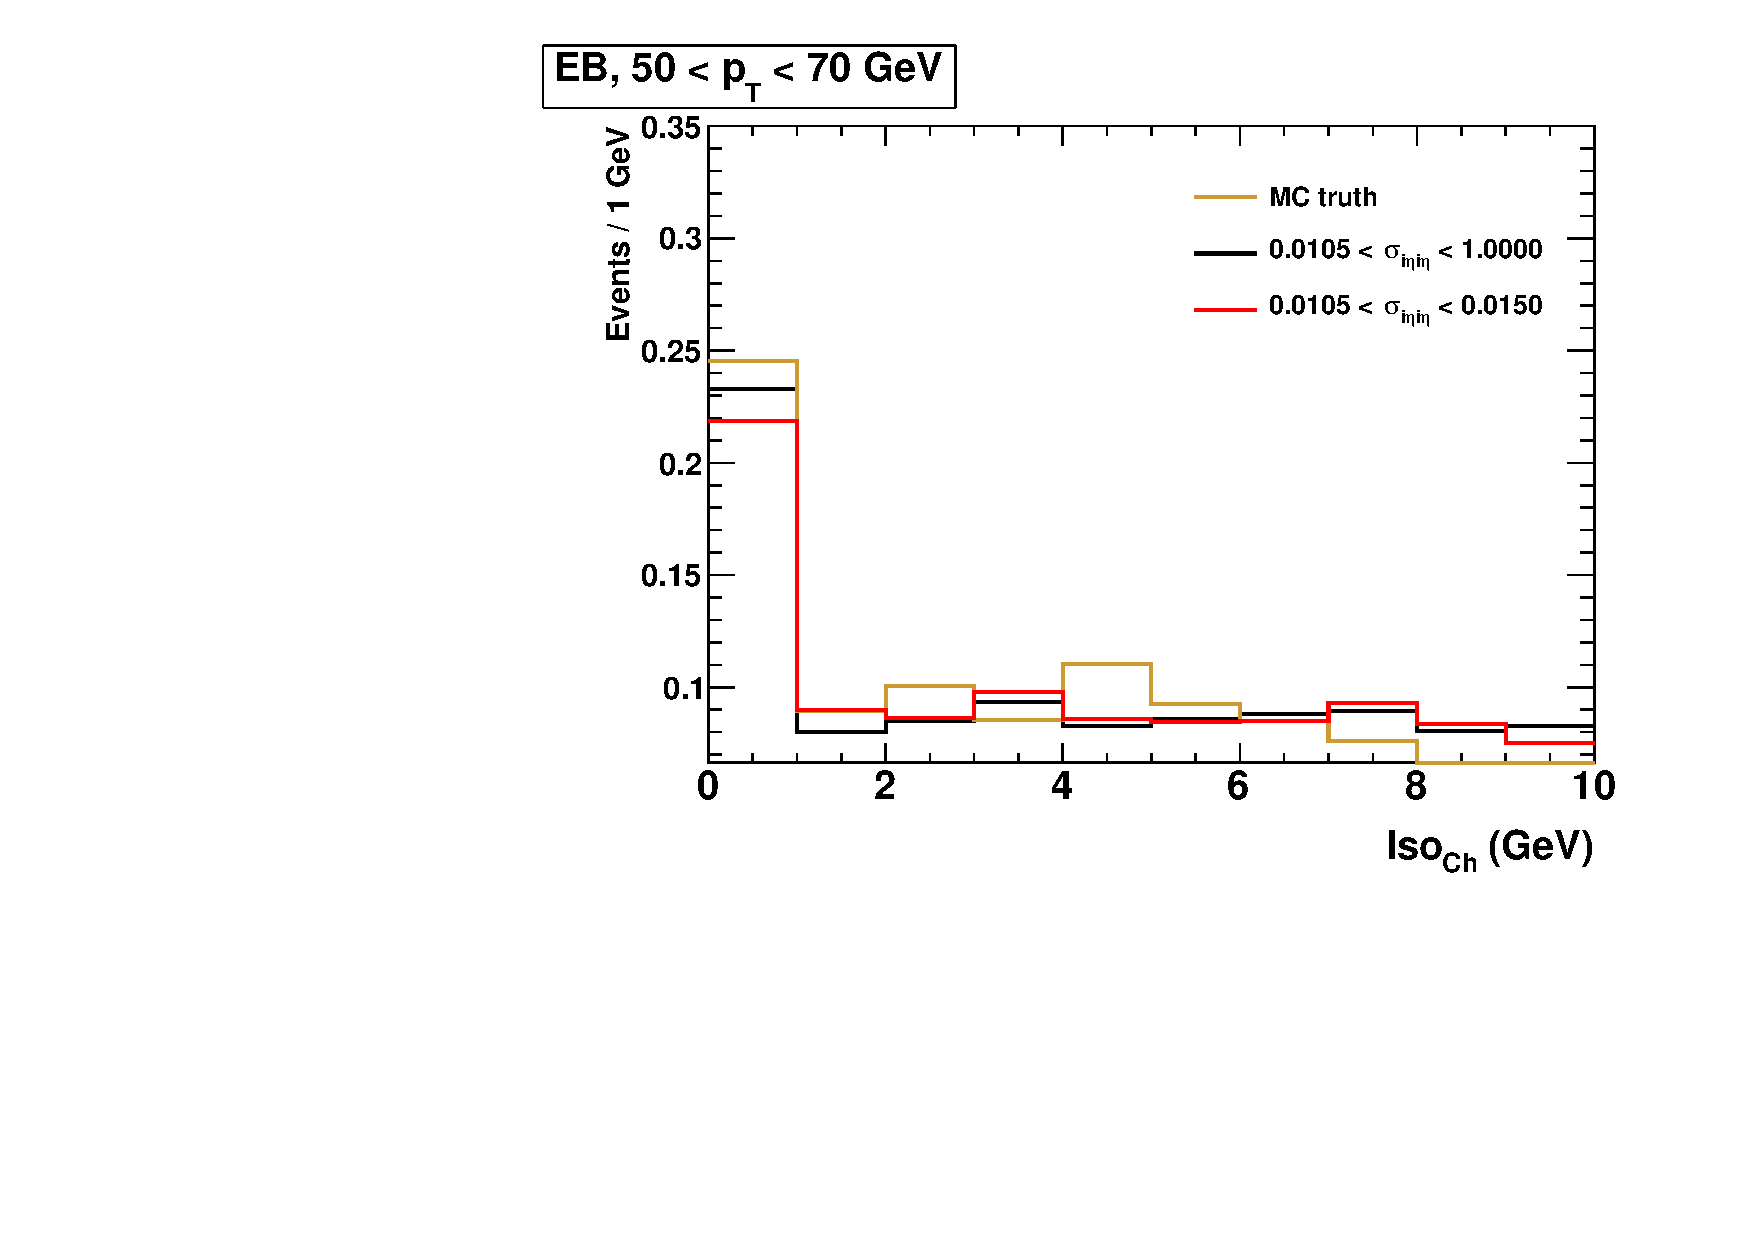
\includegraphics[scale=0.29]{figures/closure_test_fake_template_chIso_EB_pt50To70_sample_all.pdf} \\
		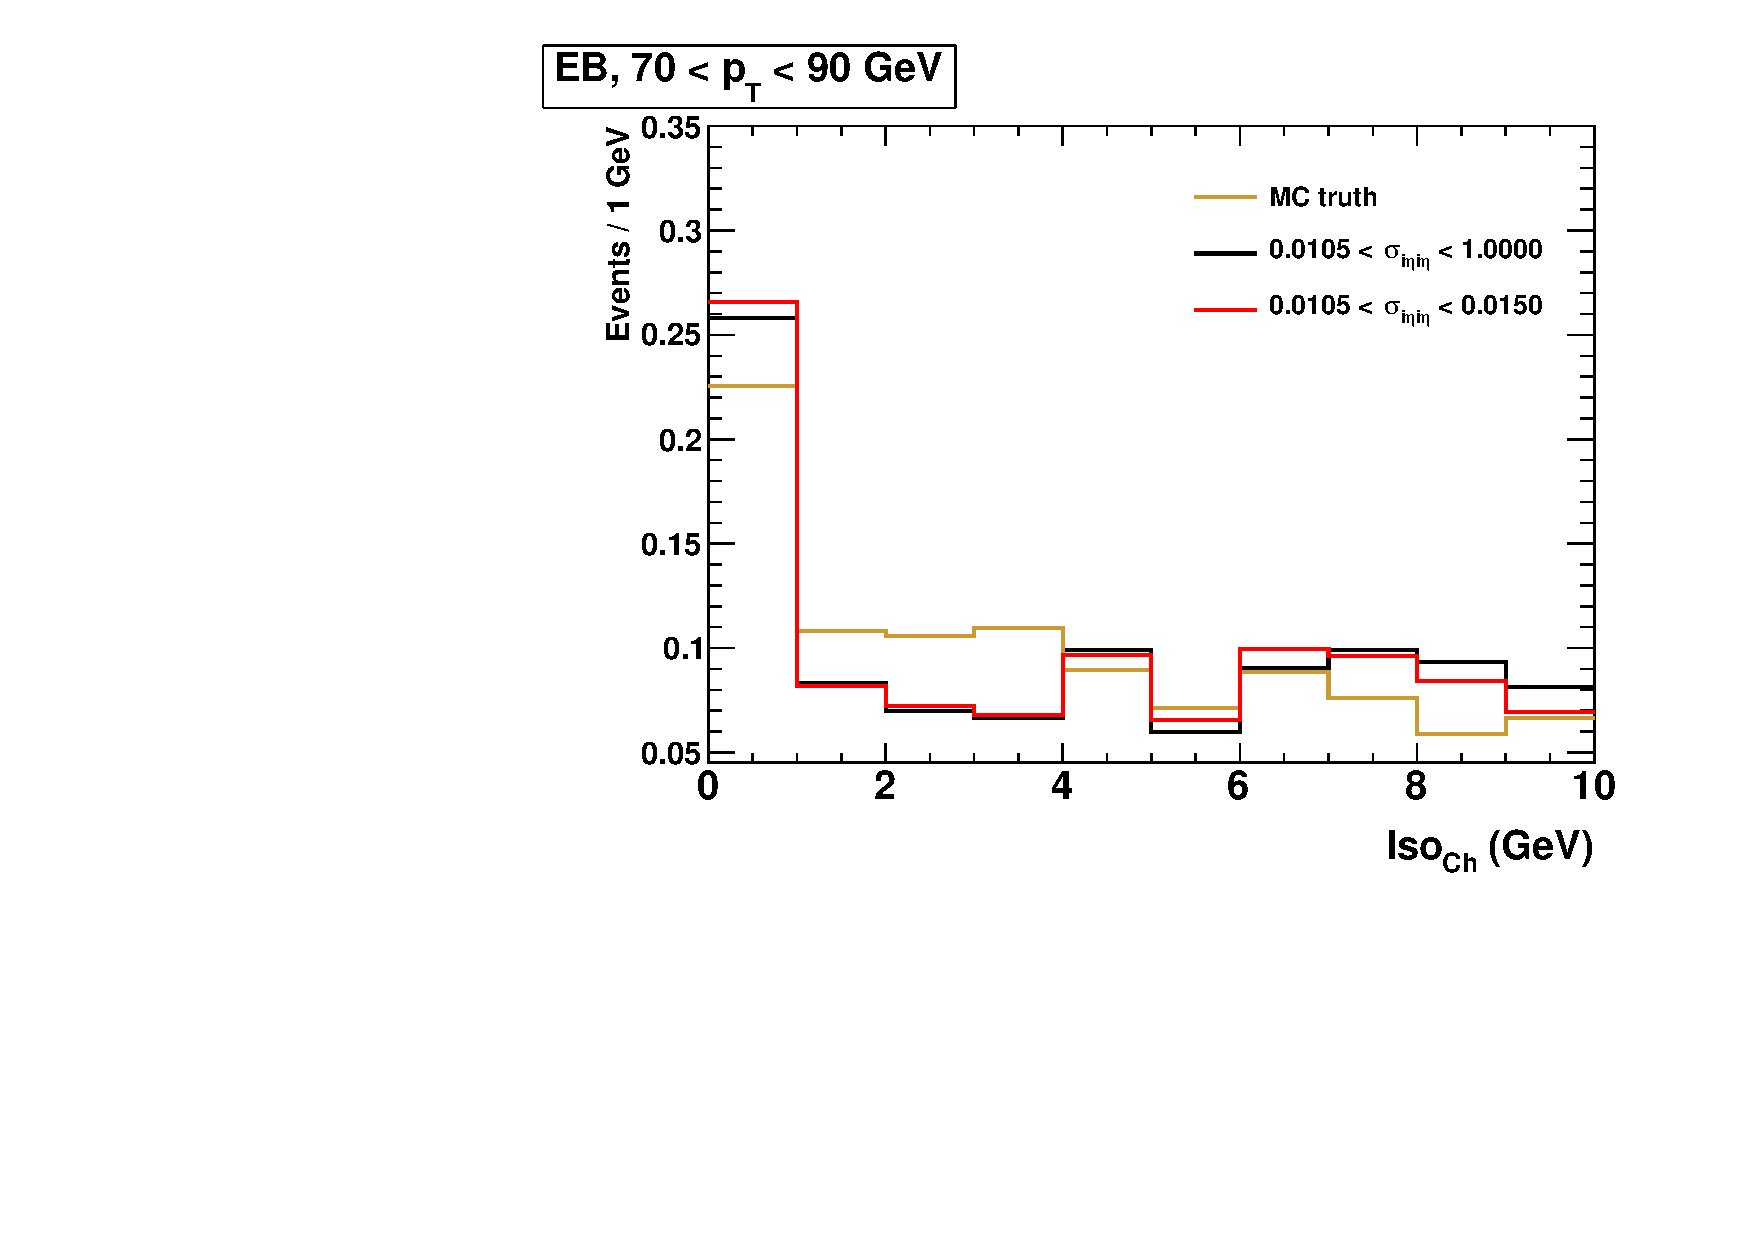
\includegraphics[scale=0.29]{figures/closure_test_fake_template_chIso_EB_pt70To90_sample_all.pdf} \\
		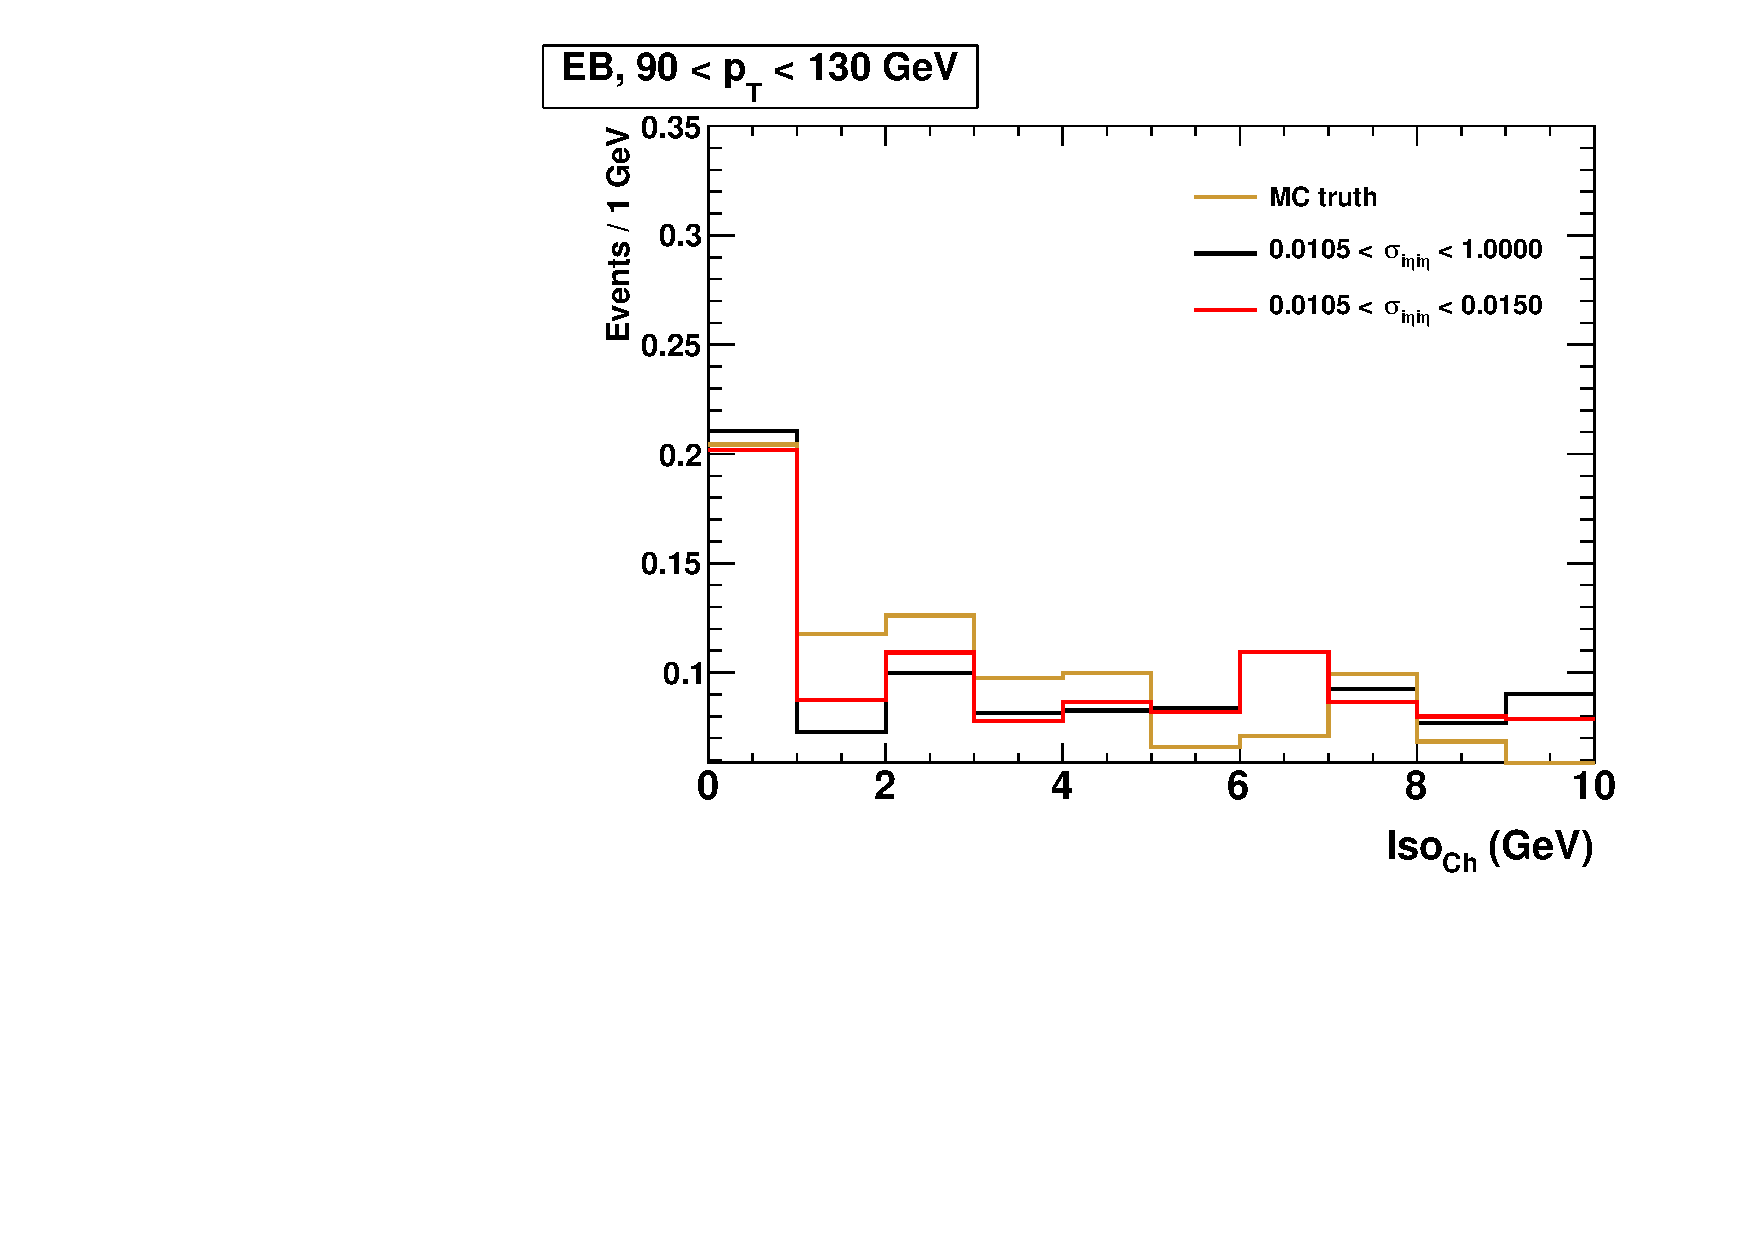
\includegraphics[scale=0.29]{figures/closure_test_fake_template_chIso_EB_pt90To130_sample_all.pdf} \\
		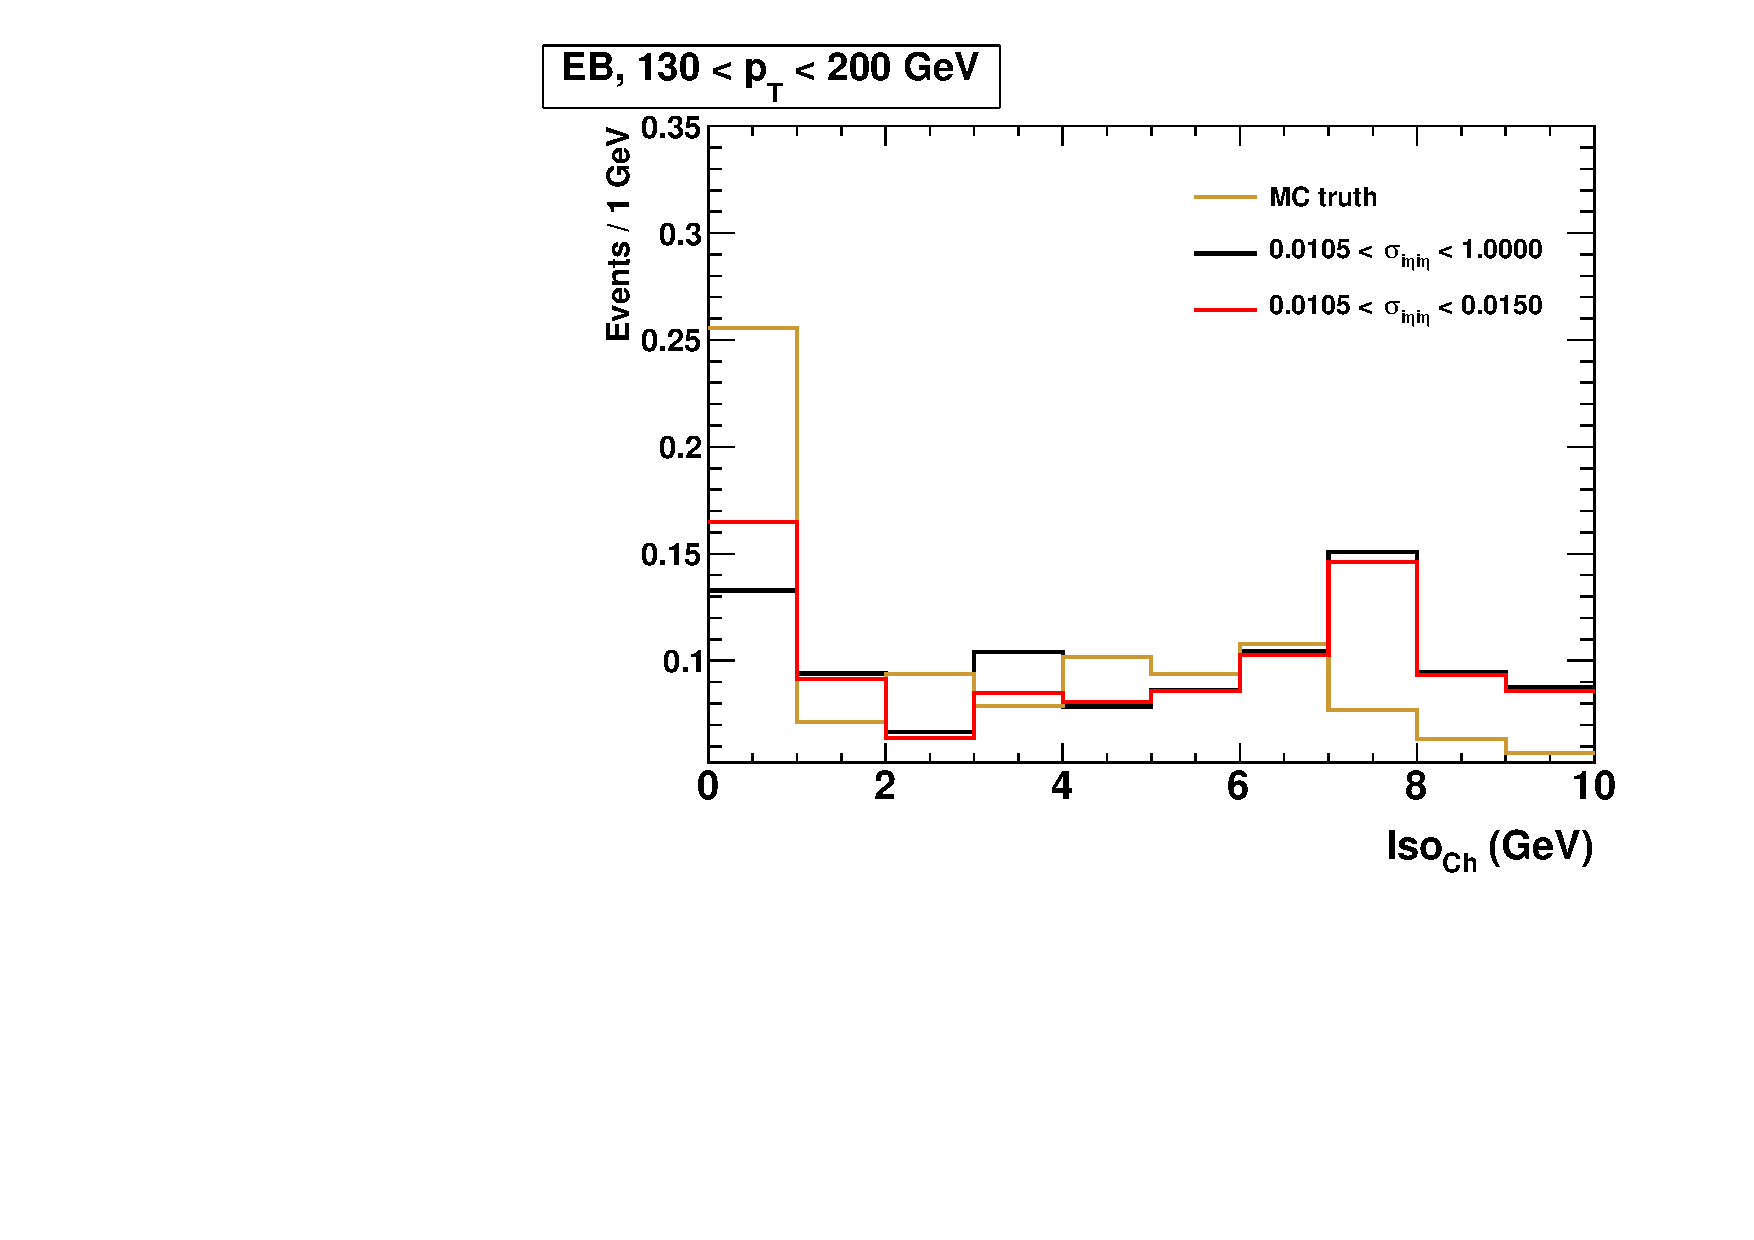
\includegraphics[scale=0.29]{figures/closure_test_fake_template_chIso_EB_pt130To200_sample_all.pdf} \\
		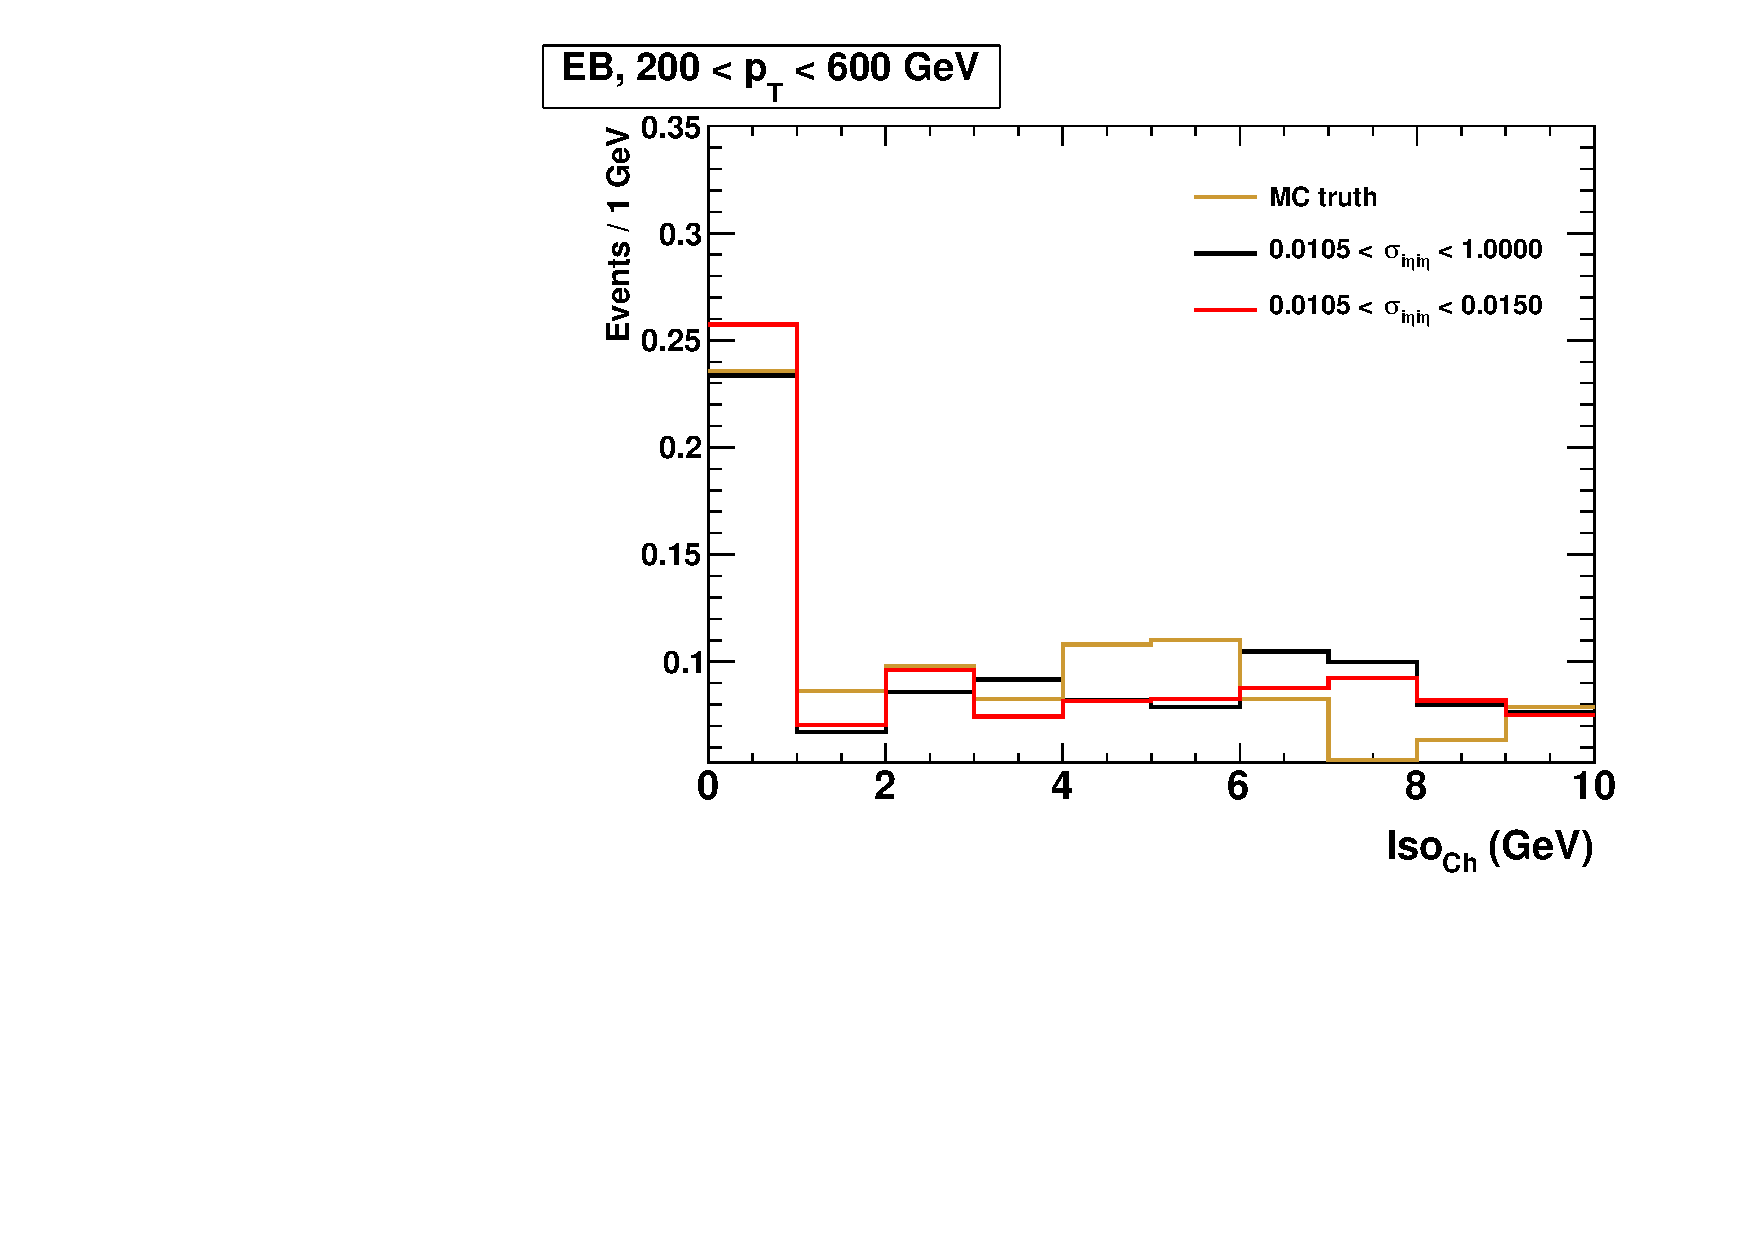
\includegraphics[scale=0.29]{figures/closure_test_fake_template_chIso_EB_pt200To600_sample_all.pdf} \\
		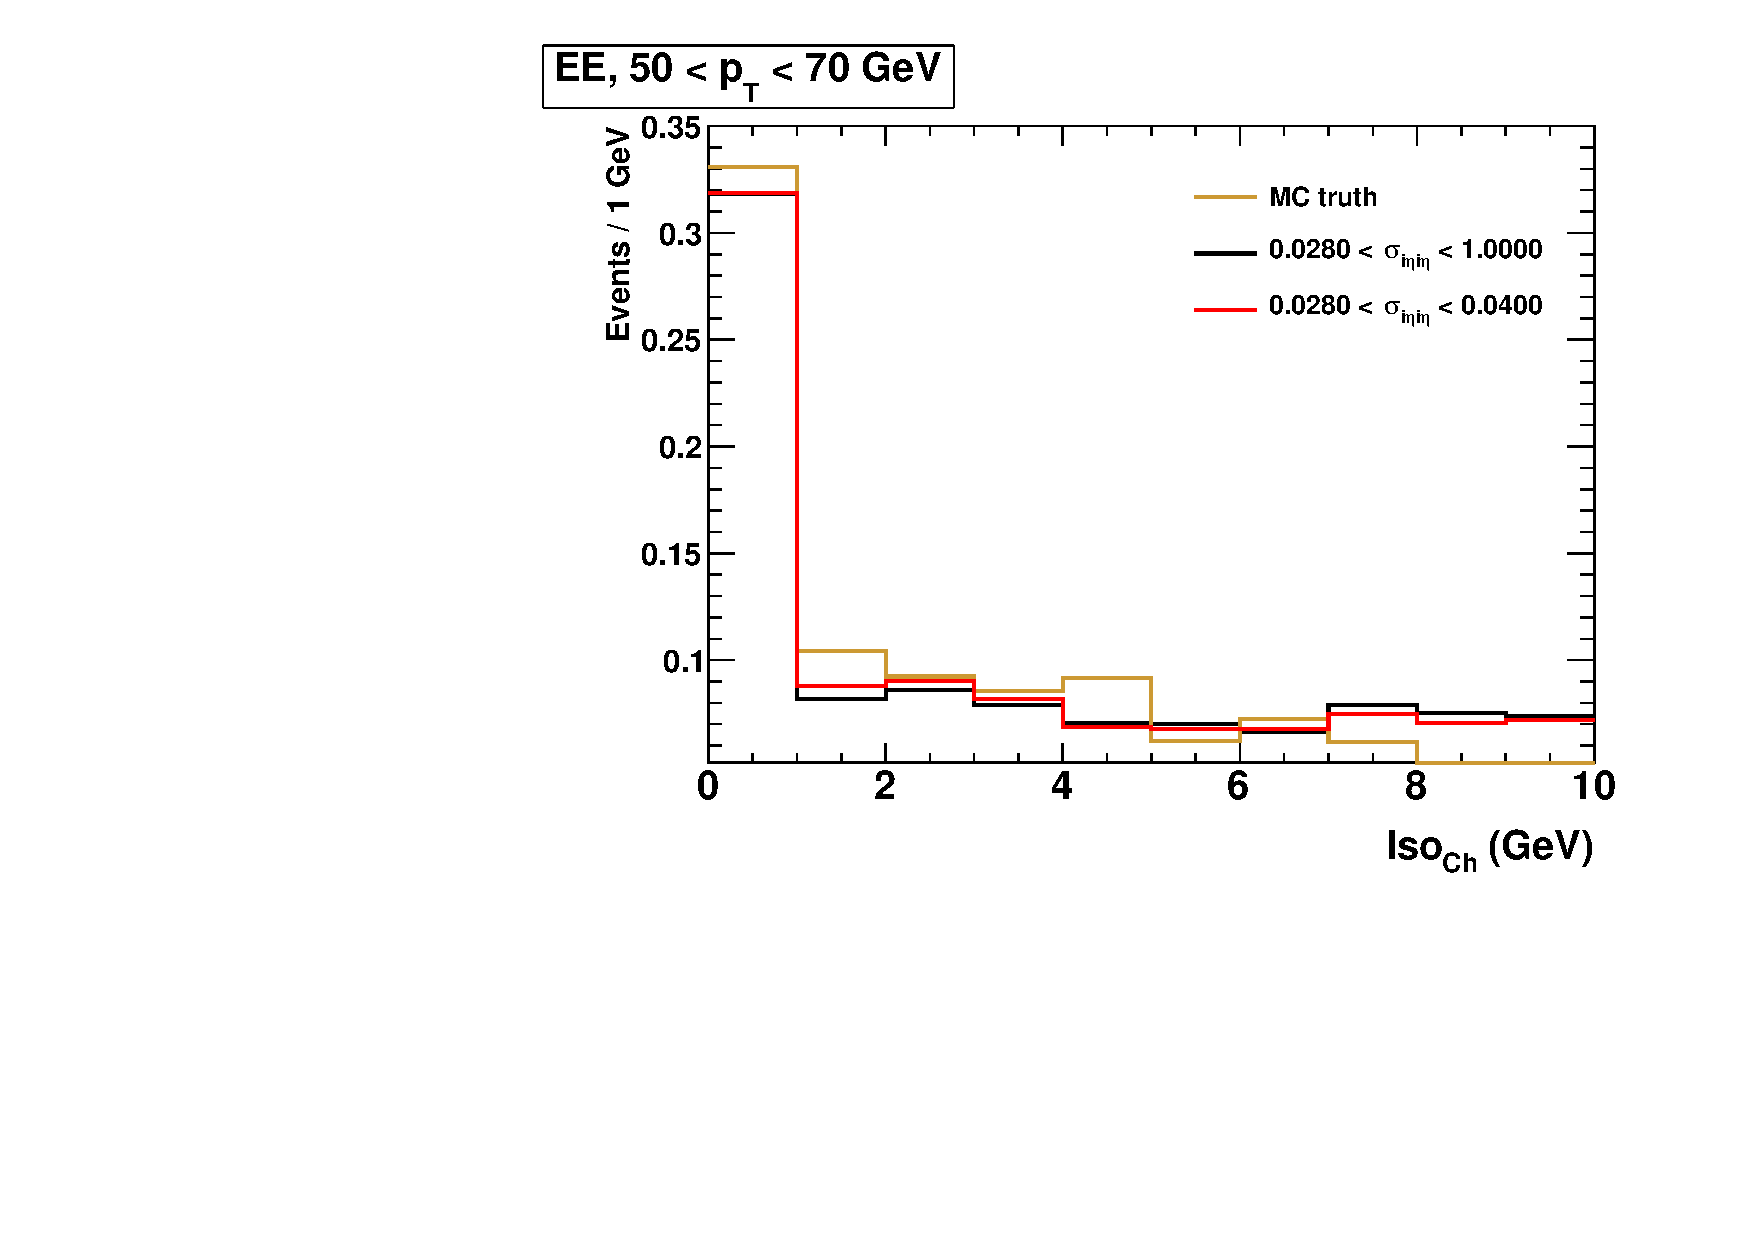
\includegraphics[scale=0.29]{figures/closure_test_fake_template_chIso_EE_pt50To70_sample_all.pdf} \\
		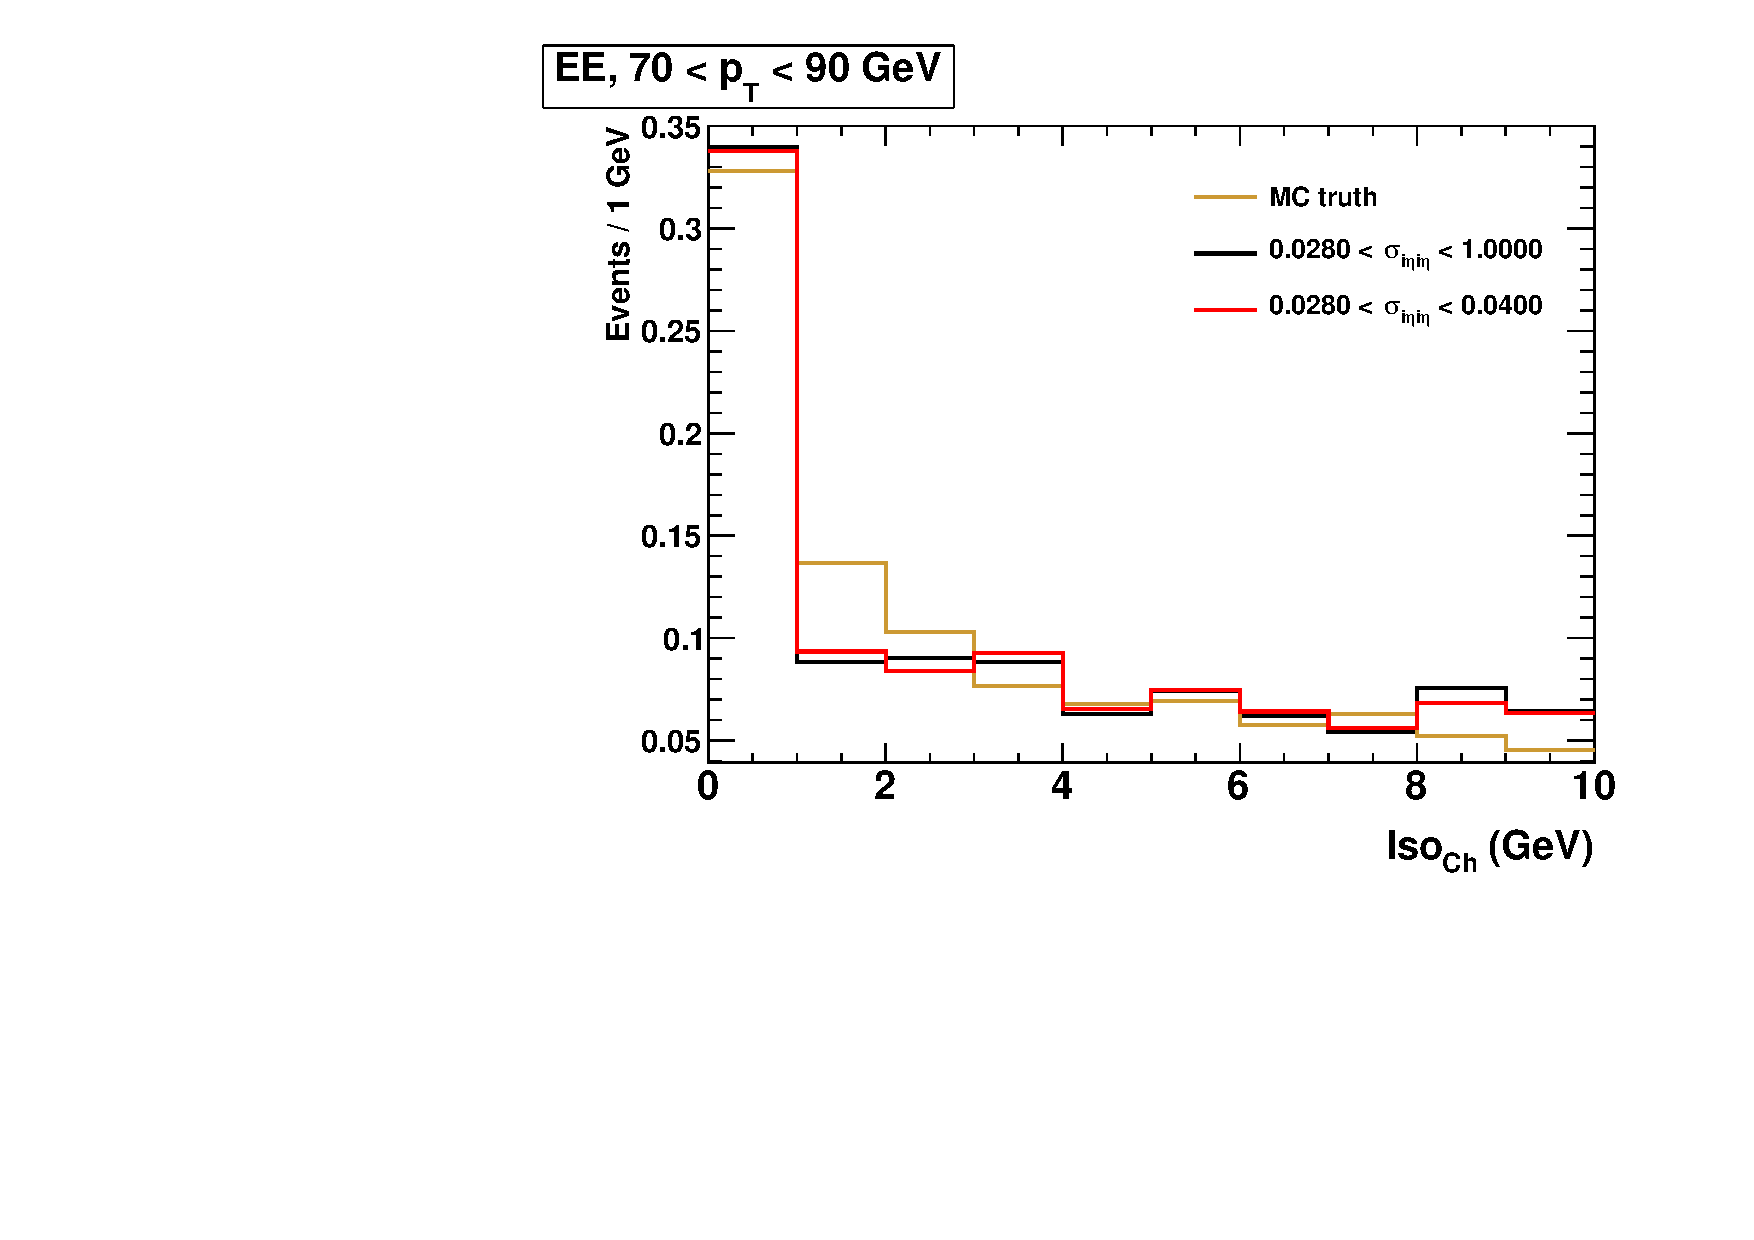
\includegraphics[scale=0.29]{figures/closure_test_fake_template_chIso_EE_pt70To90_sample_all.pdf} \\
		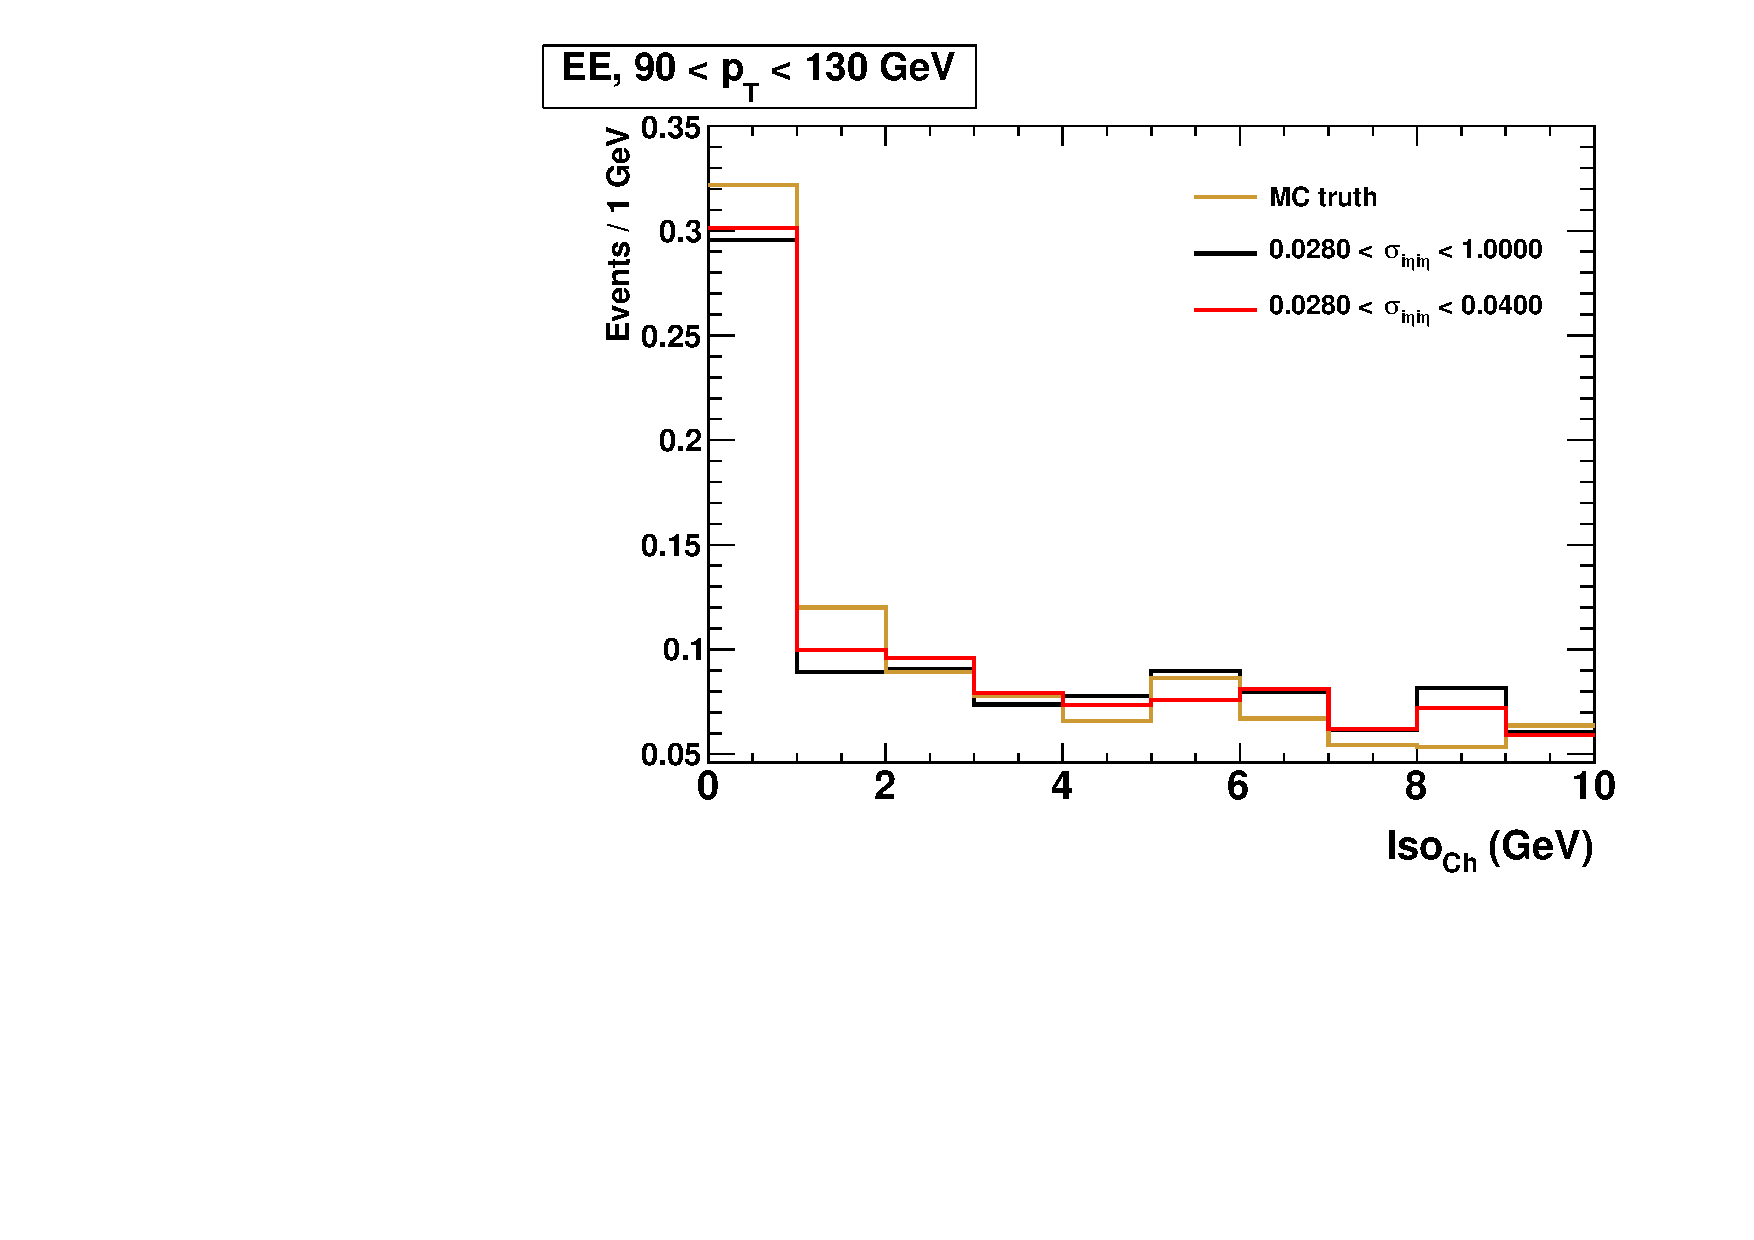
\includegraphics[scale=0.29]{figures/closure_test_fake_template_chIso_EE_pt90To130_sample_all.pdf} \\
		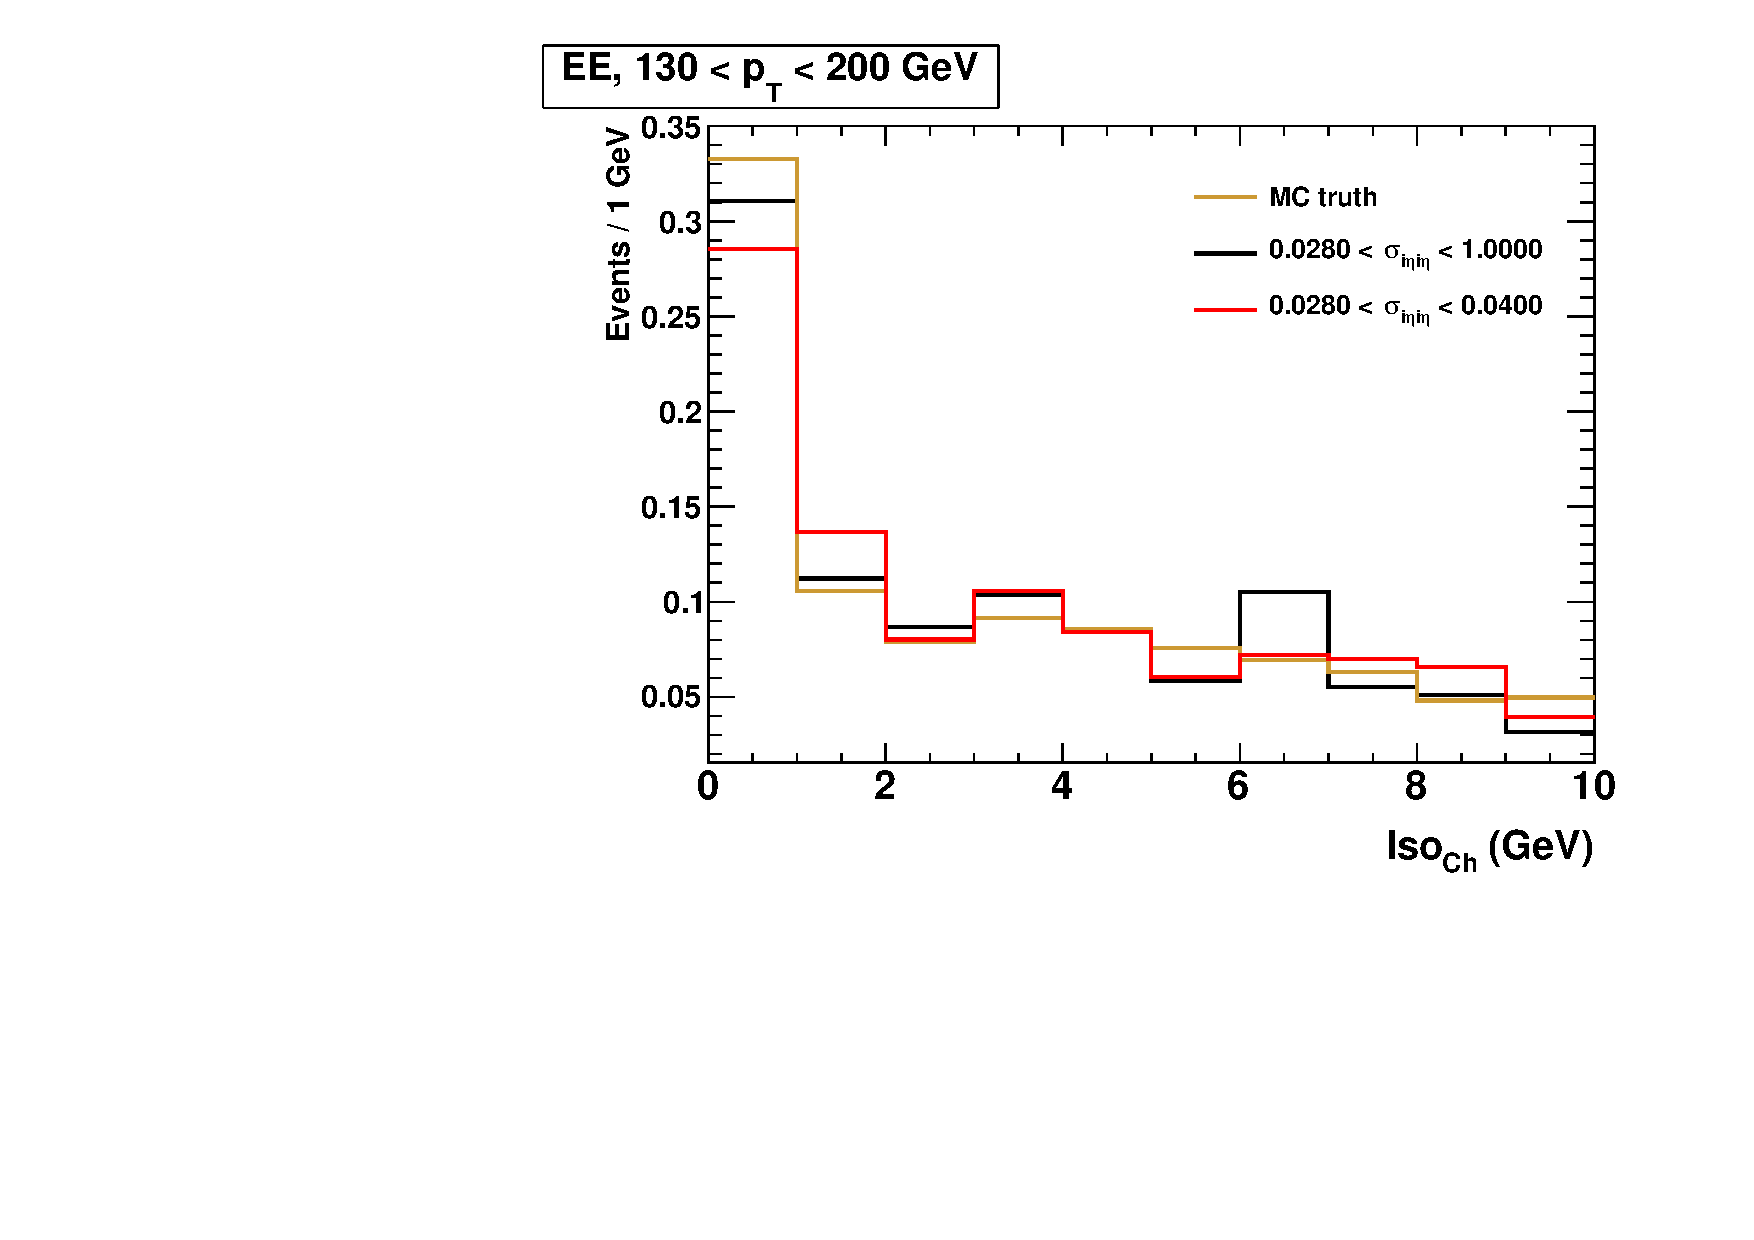
\includegraphics[scale=0.29]{figures/closure_test_fake_template_chIso_EE_pt130To200_sample_all.pdf} \\
		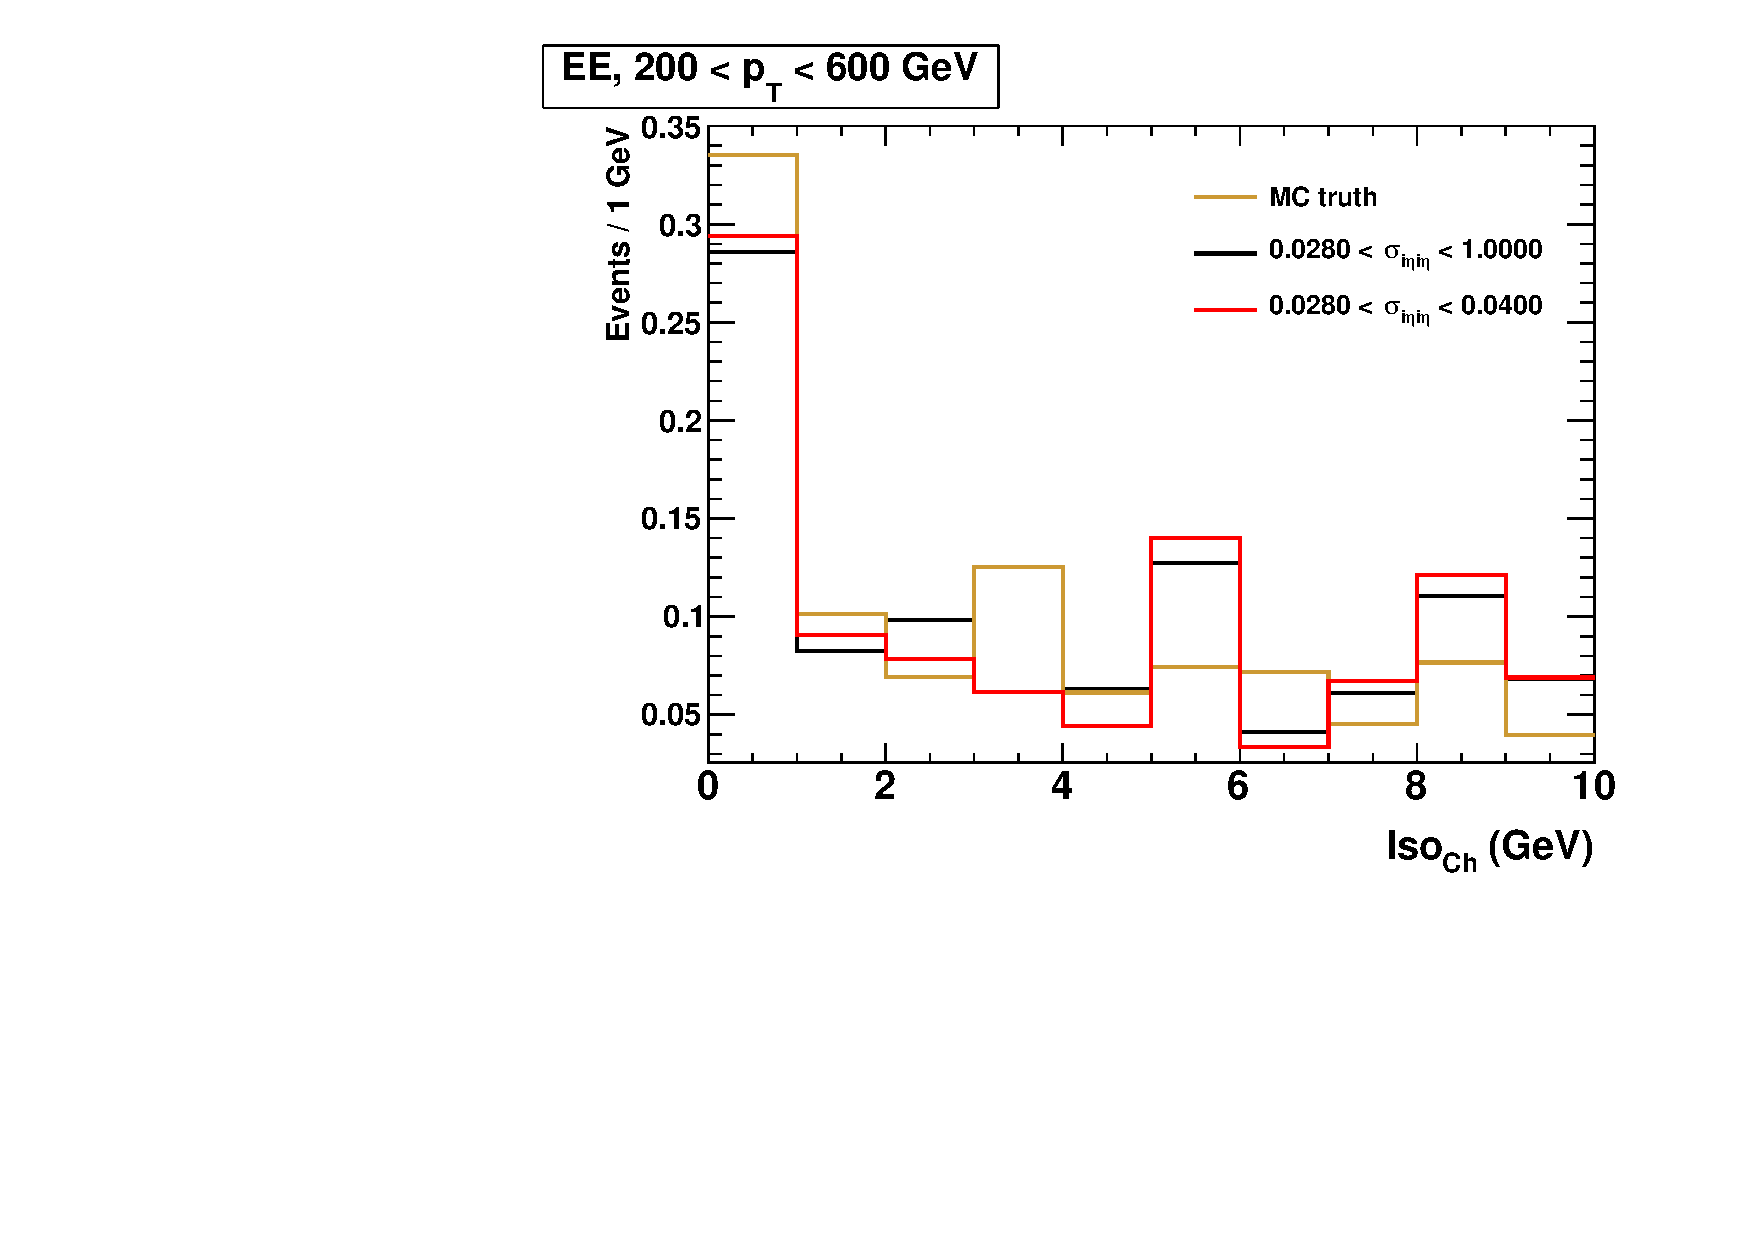
\includegraphics[scale=0.29]{figures/closure_test_fake_template_chIso_EE_pt200To600_sample_all.pdf} \\
    \end{multicols}
	\vspace{-0.5cm} % temp fix for removing extra white space
  	\caption{Fake templates in \chiso from simulation in the EB (left) and EE (right) categories for various \pt bins, shown in the rows.}
  	\label{fig:all_mc_chiso_fake_templates}
\end{figure}
